%--------------------------------------------------------------------------
% THESIS: The MAIN thesis file from which all other things are included.
%--------------------------------------------------------------------------

% Include the header which includes packages, the Acadia style and definitions.

%---------------------------------------------------------
% Header: This file includes all the packages and custom definitions
% we have used in this example thesis.
%----------------------------------------------------------

% Uncomment the following line if, for some reason, you want a PDF 1.4
% document, rather than (at time of writing) PDF 1.5.
% \pdfminorversion=4

\documentclass[12pt,twoside,openright]{report}

% With these lines, when one tried to copy/paste from AR it does The
% Right Things for ligatures.
\input{glyphtounicode}
\pdfgentounicode=1

%---------------------
% START: Packages
%---------------------
\usepackage{textcomp}
\usepackage[latin1]{inputenc}
\usepackage{amsmath}
\usepackage{amsfonts}
\usepackage{amssymb}
\usepackage{amsthm}
\usepackage{graphicx}
\usepackage{soul}
\usepackage{listings}
\usepackage{subfig}
\usepackage{verbatim}
\usepackage{alltt}
\usepackage{multicol}
\usepackage{placeins}
\usepackage{enumitem}

% There are used in the graphics chapter.
% You can delete the following two lines if you use no tikz/pgf graphics
% in your thesis.
\usepackage{tikz}
\usepackage{tikz-er2}
\usepackage{pgfplots}

% Load the natbib citation package: set the citations to be numerical
% with square brackets separated by commas.
\usepackage[numbers,square,comma]{natbib}

% Now include the Acadia thesis style
\usepackage{acadia-hon-thesis}

% Load the hyperref package.
% The options tell it to (a) use hyper-links to pages with Roman
% numerals that are different than pages with Arabic numbers, and
% (b) tell Adobe reader to show a page number matching the thesis page
% number (rather than sequentially numbering the PDF pages from 1).
\usepackage[plainpages=false,pdfpagelabels]{hyperref}

% The information in the first three lines here goes into the PDF
% document properties.
% The rest of the lines define options related to hyper-links.
% colorlinks: typeset links in the given colours
%	      (otherwise an ugly box is drawn around the links, although
%	       it is only seen on the screen, not in printed copies)
% A newer option (since May 2011) would be to just use the hidelinks option.
% Note: pdfprintscaling=None should discourage Adobe reader from wanting to
% scale your pages to fit printable area when you print from Adobe reader.
\hypersetup{%
    pdftitle={PUT YOUR THESIS TITLE HERE},
    pdfauthor={PUT YOUR NAME HERE},
    pdfkeywords={PUT ANY KEYWORDS HERE},
    colorlinks = true,
    linkcolor = black,
    anchorcolor = black,
    citecolor = black,
    filecolor = black,
    urlcolor = black,
    pdfprintscaling=None
}


% Load the algorithm/mic packages and use chapter-wise numbering
\usepackage[chapter]{algorithm}
\usepackage{algorithmic}


% JD addition:
% The url package does not, by default, allow breaks at '-'.  Change this
% by adding \do\- to this macro.  If you don't want breaks at '-' in URLs,
% just comment out or delete these lines:
\def\UrlBreaks{\do\.\do\@\do\\\do\/\do\!\do\_\do\|\do\;\do\>\do\]\do\-%
               \do\)\do\,\do\?\do\'\do+\do\=\do\#}%


%---------------------
% END: Packages
%---------------------
%\bibliographystyle{alpha}   % make citations look like [Smi91], not [12]
\bibliographystyle{plainnat}   % Default boring and almost useless number.

% The depth of the table of contents: change the MAXIMUM depth of
% citations in your table of contents.
\setcounter{tocdepth}{6}

%
% Some definitions of commands used in this thesis
%

% For instance, if you have an acronym you like to use, then define a
% command, it's faster and if the acronym changes you only have to
% change it in one place.
\def\sysacro{SPECIALACRONYM}

% Allow us to change the margins easily and at will
\newenvironment{changemargin}[2]{%
  \begin{list}{}{%
    \setlength{\topsep}{0pt}%
    \setlength{\leftmargin}{#1}%
    \setlength{\rightmargin}{#2}%
    \setlength{\listparindent}{\parindent}%
    \setlength{\itemindent}{\parindent}%
    \setlength{\parsep}{\parskip}%
  }%
  \item[]}{\end{list}}

%setup the default format of listings
\lstset{
    basicstyle=\footnotesize,
    numbers=left,
    xleftmargin=5mm,
    linewidth=\textwidth,
    breaklines,
    frame=tb,
    frameround=fttt
}

% A new definition style
\newtheoremstyle{defstyle}	% name
    {3pt}			% Space above
    {3pt}			% Space below
    {}				% Body font
    {}				% Indent amount
    {\itshape}			% Theorem head font
    {:}				% Punctuation after theorem head
    {.5em}			% Space after theorem head
    {}		% Theorem head spec (can be left empty,meaning 'normal�)
\theoremstyle{definition}
\newtheorem{definition}{Definition}[chapter]


% Change comment style for algorithms
\renewcommand{\algorithmiccomment}[1]{/*#1*/}
% Change Require: to Input: for algorithms
\renewcommand{\algorithmicrequire}{\textbf{Input:}}
% Change Ensure: to Output: for algorithms
\renewcommand{\algorithmicensure}{\textbf{Output:}}


\pgfplotsset{compat=1.14}
\begin{document}

    % PRELIMINARIES: This is the file you will use to setup your
    % name, date, advisor, etc. 
    %---------------------------------------------------------
% Preliminaries: Set up your own details in this file!
%----------------------------------------------------------

% Don't forget to remove the ()s in ALL of these "personalization" lines.

\title{Development of a comprehensive learning management system designed for
computer science department}

\author{Bailin He}
\dept{Computer Science}   % E.g., Physics, Computer Science,
\deptOrSchool{School}
\degree{Computer Science}  % E.g., Science, Arts, ...

\submissionMonth{July}	    % OR WHATEVER MONTH YOU ACTUALLY SUBMIT IN
\submissionYear{2018}
\copyrightYear{2018}		    % Probably the same as submissionYear.

% Use a "~" after the "r." of "Dr." so that TeX doesn't think you have
% ended a sentence (at which point it gives extra space).
\supervisor{Dr. James Diamond}

% Remove the '%' from the next line and fill in the name if desired.
%\cosupervisor{(Dr.~Your Other Supervisor)}

\headOrDirector{Dr. Darcy Benoit}
% If the head or director is an ``acting'' head or director, uncomment
% the next line (i.e., delete the '%'):
% \justActing

% You will have to ask around to find out the name of the person
% to put here... it changes from year to year.
\honoursCommittee{Dr. Matthew Lukeman} % To end of August

%-------------------------------------------------------------------------

% This outputs the title page, the approval page and the copyright page.
\firstThreePages

%-------------------------------------------------------------------------
% Now write your acknowledgements (if any).
% If you wish to acknowledge no-one, delete or comment-out the
% next few lines.

\Acknowledgments

%-------------------------------------------------------------------------

% This outputs the table of contents, lists of figures, tables, ...

\tocAndSuch

%-------------------------------------------------------------------------

\prefacesection{Abstract}

This thesis presents a learning management system (LMS) written in Python using
the Django web framework. This system is designed specifically for computer science
and mathematics instructors and students to ease the process of submitting and,
more importantly, the process of grading assignments, with a built-in code
testing module for programming assignments to build and run all students'
submitted solutions and provide informative test results for students and
markers, as well as features like syntax highlighting, Markdown input and \TeX\
notation input for mathematical equation rendering for markers and instructors
to comment on the students' assignments.


%-------------------------------------------------------------------------

% Don't mess with this line!
\afterpreface


    % CHAPTER CONTENT START
    % Replace all the lines from here down to ``CHAPTER CONTENT END''
    % with a collection of ``\include{XYZ}'' lines, where each such XYZ
    % is the name of a text file holding (for example) one chapter of
    % your thesis.
    % If you have appendices you need that ``\appendix'' line BEFORE
    % you \include your appendices.
    
%-----------------------------------------------------------------------------
% Chapter: Introduction
%-----------------------------------------------------------------------------

\chapter{Introduction}
\label{chap:INTRO}

Many courses in Computer Science involve programming in one or more programming
languages.
The nature of programming assignment evaluation
involves processes like code testing, debugging, commenting, and code style
checking.
This makes the evaluation process of a programming Computer Science assignment
very different than assignments in many other disciplines.
Students would be motivated to hand in a higher quality assignment
if more information were provided shortly after their assignments were
submitted.
A learning management system (LMS) that can automatically test the
submitted assignments and have the results provided for both the markers and
the students is desirable.

\section{Background}

Acadia University currently uses the Moodle Learning System (also known at 
Acadia University as ACORN) as the default LMS.
This system works well for most of the courses, however, it has shortcomings
when it comes to Computer Science programming assignments.
As evidenced by considering the nature of programming source code files,
the Moodle LMS lacks certain features that are essential to Computer Science
students and instructors,
including, but not limited to, monospace text font for plain text
file display, programming language detection, and syntax
highlighting for source code file display.
Moreover, it is not uncommon for Computer Science markers and instructors
to want to put mathematical equations or formulas into their comments on
students' assignments. The only ways to do this with the Moodle
LMS are to draw the equations or formulas by hand with the
pointing device of the computer (i.e., computer mouse, trackpad), write
them in \emph{HTML} code,
or create them in another program and then insert them into the Moodle LMS as
an image. All three of these methods are time-consuming.

\medskip

The \emph{Course2000} course system, designed by former Acadia Computer Science
professor Dr.~Rick Giles, is a good choice
of alternative LMS to the Moodle Learning System.
It has been the
default LMS for one Computer Science course, \emph{COMP 2103: Programming 3},
for over 16 years.
With a recent addition to the system,
the \emph{Visual Mark} module,
designed and integrated by former student Tim Cooper,
the \emph{Course2000} system has proven itself
to be very capable of handling Computer Science assignments.
However, with more
and more modifications applied to the system over the years, maintaining
this system has become more and more difficult.
Further, the amount of work required to add new features to the
system (especially the key features this thesis intends to achieve,
see Section~\ref{FEATURES}) has increased dramatically
due to its legacy codebase.
For example, the whole system front-end of the \emph{Course2000} LMS was built
with an \emph{HTML} feature called \emph{framing}, which is an obsolete feature
and has been dropped in \emph{HTML5}~\cite{framing};
as a result, a lot of the desired changes to the \emph{Course2000} system would
require a complete rewrite of the entire system front-end.

\section{Course2018}
Influenced by the \emph{Course2000} system, the goal of this project is to
develop a secure and dynamic LMS with functionalities designed specifically for
Computer Science instructors and students.
These functionalities are mainly focused on
providing informative feedback on programming assignments to both students
and instructors for the purpose of easing the process of learning as well as
evaluation.
Simplicity of the overall system design is an important goal of this project;
every task the system 
performs can be done efficiently for both the users and the server,
and the future development as well as maintenance will not be too difficult.

\subsection{Key features}
\label{FEATURES}
The \emph{Course2018} LMS contains the following functionalities.

\subsubsection{Source code management}
The \emph{Course2018} LMS provides the ability for students to manage
their source code more efficiently and more professionally. With features such
as source code version control, students and instructors are now able
to view the history of every source code file, and more importantly, compare
the changes between different versions of each file.

\subsubsection{Souce code display}
Source code display is one fundamental feature of the \emph{Course2018} LMS,
which provides better readability of source code files for the users.
A syntax highlighter is included in the system for over 300 programming
languages~\cite{ApygmentsLangs}.

\subsubsection{Automated tests for programming assignments}
When a programming assignment is submitted by a student with \emph{Course2018},
a program associated with the submitted source code file(s) will be built
(if required).
This program
will then be executed with the sample input data provided to the system
by the instructor.
As soon as the program execution is finished, 
the output of the program will be compared with the sample output data~(also
provided by the instructor) and
an informative test result will be generated for the relevant parties~(i.e.,
the student who submitted the assignment, the markers, and the
instructor).

\subsubsection{Informative assignment feedback}
The key to providing informative assignment feedback comments in computer
science assignments (especially programming assignments) is to make sure the
comments are well formatted.
Therefore, an easy-to-use plain text markup language called \emph{Markdown}
is introduced to the \emph{Course2018} marking system. This markup language was
designed to be automatically converted to \emph{HTML} format.
Also, \emph{Markdown} is
widely used by well-known websites including \emph{GitHub} \cite{CgitHubMarkDown}
and \emph{Stack Overflow} \cite{stackOverflowMarkdown}.
An improvement has been made to support mixed
input of \emph{Markdown} and \TeX\ mathematical notation.

\subsubsection{Powerful built-in text editor}
With the enhanced assignment feedback solution mentioned above, a powerful
text editor that supports syntax highlighting, and custom key-bindings is also
integrated to the \emph{Course2018} LMS in order to ease the actual process of
typing for the markers and instructors.
    
%-----------------------------------------------------------------------------
% Chapter: Introduction
%-----------------------------------------------------------------------------

\chapter{Requirements Analysis}
\label{chap:REQS}

The first step of this project was performing an overall requirements analysis
in order to determine the general needs of the \emph{Course2018} LMS.\ \ 
In this chapter, some key requirements will be investigated for their
feasibility and expectations.
Depending on the specifications of the requirements, they are categorized into
two categories, functional requirements and non-functional requirements.

\section{Terminologies}

\subsection{Functional requirement}
\label{sec:FUNC_REQS}
A functional requirement defines a task the system needs to accomplish,
as well as the behavior of the task, which is captured and described in detail
with use cases.
These requirements will be further analyzed to design the system components
model~\cite{functionalReqs}.

\subsection{Non-functional requirement}
As opposed to functional requirements, non-functional requirements describe
non-behavioral specifications such as system performance, security, and system
environments.

\subsection{Use cases}
A use case is a series of actions performed by one or more actors interacting
with the system to accomplished a task~\cite{useCase}.

\medskip 

Use cases in this thesis are composed of the following elements:

\begin{itemize}

\item \textbf{Primary actor}:
The main user (could be a person or an external system) who interacts with the
system.

\item \textbf{User story}:
A brief description of the task that the primary actor wishes to accomplish.

\item \textbf{Preconditions}:
Prerequisites to the test case,
conditions or states that must be satisfied prior to the start of the workflow.

\item \textbf{Postconditions}:
Conditions or states that must be satisfied after the workflow is finished.

\item \textbf{Triggers}:
An event (or a series of events) that starts the execution of the workflow.

\item \textbf{Basic flow}:
A step-by-step description of the detailed interactions between the actor and
the system, as well as the activities performed by the system.

\end{itemize}

\section{Functional requirements}
\label{FUNCREQS}

\subsection{User authentication}

The system must provide routines to handle activities related to user accounts
such as user login, permission checking for restricted content, and user logout.

\subsubsection{Use cases}

\begin{enumerate}
\item User login:
\begin{itemize}
\item Primary actor:
    A registered user of the \emph{Course2018} LMS.
\item User story:
    A user wishes to have access to some restricted content, therefore, he
    first needs to login to the system.
\item Preconditions:
    The user is at the login interface, and the login credentials
    (namely, username and password) are input into the corresponding fields.
\item Postconditions:
    \begin{itemize}
        \item On success: an interface with the user's information (such as courses
            in which this user is registered) will be presented to the user.
        \item On failure: a login interface with an error message will be
            presented to the user.
    \end{itemize}
\item Triggers: the \emph{Login} button is clicked.
\item Basic flow:
    \begin{enumerate}
        \item The user's login credentials are encrypted and sent to the
            server.
        \item The server compares the user's login credentials against the
            account database.
        \item If a match is found in the database, an interface with the user's
            information will be returned and the user will have access to
            some restricted content to which the user is authorized; otherwise,
            a login interface with error messages will be returned.
    \end{enumerate}
\end{itemize}

\item Permission checking:
\begin{itemize}
\item Primary actor: 
    A registered user of the \emph{Course2018} LMS
\item User story:
    The user request for accessing content for which the user may or may not
    have permission.
\need 1 in
\item Preconditions:
    \begin{itemize}
        \item The user is logged into the system.
    \end{itemize}
\item Postconditions:
    \begin{itemize}
        \item On success: an interface with the requested content will be presented
            to the user.
        \item On failure: an interface indicates that the user is unauthorized will
            be presented to the user.
    \end{itemize}
\item Triggers: the user types the request URL to the browser location field
    or clicks on a link to the URL.
\item Basic flow:
    \begin{enumerate}
        \item The request (i.e., the desired URL) of the user is sent to the server.
        \item The server checks if the request is valid, namely, if the user
            is logged in and if the user has permission to access the requested
            content.
        \item If the request is valid, an interface with the requested content will
            be returned; otherwise, an interface with an error message 
            indicating the request is unauthorized will be returned.
    \end{enumerate}
\end{itemize}

\end{enumerate}


\subsection{Course information handling}
The system shall provide instructors with abilities to manage (i.e., create, remove,
and modify) their courses.
\subsubsection{Use cases}
\begin{enumerate}
\item Create a course:
\begin{itemize}
    \item Primary actor: a registered instructor.
    \item User story: the user wishes to create a course.
    \need 2 in
    \item Preconditions: 
        \begin{itemize}
            \item The user is logged in to the system.
            \item The user is at the create course interface where a form with
                course information related fields 
                is presented to the user.
            \item The user fills in all the fields with data that may or
                may not be invalid.
        \end{itemize}
    \item Postconditions:
        \begin{itemize}
            \item On success: a summary interface of the course the user created
                will be presented.
            \item On failure: the same create course interface with error
                messages indicating which fields were filled with invalid data
                will be presented.
        \end{itemize}
    \item Triggers: the \emph{Create} button is clicked.
    \item Basic flow:
        \begin{enumerate}
            \item The form with the update course information is encrypted and
                sent to the server.
            \item The server validates the form data for errors including,
                but not limited to,
                invalid input format
                (i.e., invalid date/time field input format,
                input text length is greater than the maximum text length
                allowance defined in the database),
                conflicts (i.e., a course with the same identifier  
                already exists for that academic year),
                and numbers out-of-range.
            \item If the validation fails, the same create course interface
                with error messages will be returned; otherwise, the server will
                execute the routines to create a course with the submitted 
                information and have the summary interface of that course prepared
                and returned.
        \end{enumerate}
\end{itemize}

\item Update course information:
\begin{itemize}
    \item Primary actor: a registered instructor.
    \item User story: the user wishes to update the information of one course.
    \item Preconditions:
        \begin{itemize}
            \item The user is logged in to the system.
            \item The user has previously created a course.
            \item The user is at the manage course interface for the course to
                be modified, where a form with
                the course's existing information pre-filled is presented.
            \item The user has updated some of the fields in the form with some
                new data that may or may not be valid.
        \end{itemize}
    \item Postconditions:
        \begin{itemize}
            \item On success: the manage course interface where a form with
                the course's updated information pre-filled will be presented
                to the user.
            \item On failure: the manage course interface with error messages
                indicating which fields were filled with invalid data will be
                presented to the user.
        \end{itemize}
    \item Triggers: the \emph{Save Changes} button is clicked.
    \item Basic flow:
        \begin{enumerate}
            \item The form with course-related data is encrypted and sent to
                the server.
            \item The server validates the form data for errors including,
                but not limited to,
                invalid input format
                (i.e., invalid date/time field input format,
                input text length is greater than the maximum text length
                allowance defined in the database),
                conflicts (i.e., a course with the same identifier  
                already exists for that academic year),
                and numbers out-of-range.
            \item If the validation failed, the same create course interface
                with error messages will be returned; otherwise, the server will
                execute the routines to update the course with the submitted 
                information and have the new manage course interface with the
                updated course data prepared and returned.
        \end{enumerate}
\end{itemize}

\item Remove a course:
\begin{itemize}
    \item Primary actor: a registered instructor.
    \item User story: the user wishes to remove a course from the system.
    \item Preconditions:
        \begin{enumerate}
            \item The user is logged in to the system.
            \item The user has previously created a course.
            \item The user is at the manage course interface for the course
                to be removed.
            \item The user clicked the \emph{Delete Course} button and a
                confirmation dialogue is presented.
        \end{enumerate}
    \item Postconditions:
        The course, along with all relevant data (such as registered students,
        assignments, and student grades) will be removed from the system
        database.
    \item Triggers: the \emph{Confirm} button on the confirmation dialogue is
        clicked.
    \item Basic flow:
        \begin{enumerate}
            \item A \emph{delete} request with the course identifier is encrypted
                and sent to the server.
            \item The server examines the request and makes sure the user is
                authorized to perform such an activity.
            \item If the request is valid, the course along with all its
                relevant data will be removed from the system database.
        \end{enumerate}
\end{itemize}

\end{enumerate}

\subsection{Assignment information handling}
The system shall provide the ability for instructors to manage (i.e., create,
remove, and modify) the assignments of their courses, as well as the ability for
students to submit and view those assignments.

\subsubsection{Use cases}
\begin{enumerate}
\item Create an assignment:
\begin{itemize}
    \item Primary actor: a registered instructor.
    \item User story: the user wishes to create an assignment.
    \item Preconditions:
        \begin{itemize}
            \item The user is logged in to the system.
            \item The user has previously created a course.
            \item The user is at the create assignment interface where a form
                with several assignment information-related fields is
                presented to the user.
            \item The user has filled in all the fields with data that may
                or may not be valid.
        \end{itemize}
    \item Postconditions:
        \begin{itemize}
            \item On success: an summary interface of the assignment the user
                created will be presented.
            \item On failure: the same create assignment interface with error
                messages indicating which fields were filled with invalid data
                will be presented.
        \end{itemize}
    \item Triggers: the \emph{Create} button is clicked.
    \item Basic flow:
        \begin{enumerate}
            \item The form with the assignment-related data is encrypted and
                sent to the server.
            \item The server validates the form data for errors including,
                but not limited to,
                invalid input format
                (i.e., invalid date/time field input format,
                input text length is greater than the maximum text length
                allowance defined in the database),
                conflicts (i.e., an assignment with the same
                number already exists in the course),
                and numbers out-of-range.
            \item If the validation failed, the same create assignment interface
                with error messages will be returned; otherwise, the server will
                execute the routines to create an assignment with the submitted
                information and have the summary interface of that assignment
                prepared and returned.
        \end{enumerate}
\end{itemize}

\item Update assignment information:
\begin{itemize}
    \item Primary actor: a registered instructor.
    \item User story: the user wishes to update the information of one
        assignment.
    \item Preconditions:
        \begin{itemize}
            \item The user is logged in to the system.
            \item The user has previously created a course.
            \item The user has previously created an assignment for that course.
            \item The user is at the summary interface of the assignment to be
                modified, where a form with the assignment's existing
                information pre-filled is presented.
            \item The user has updated some of the fields in the form with some
                new data that may or may not be valid.
        \end{itemize}
    \item Postconditions:
        \begin{itemize}
            \item On success: the same assignment summary interface with the updated
                information will be presented to the user.
            \item On failure: the same assignment summary interface with error
                messages indicating which fields were filled with invalid data will
                be presented to the user.
        \end{itemize}
    \item Triggers: the \emph{Save Changes} button is clicked.
    \item Basic flow:
        \begin{enumerate}
            \item The form with the updated assignment information is encrypted
                and sent to the server.
            \item The server validates the form data for the same errors
                mentioned in the previous use case.
            \item If the validation failed, the same assignment summary interface
                with error messages will be returned; otherwise, the server will
                execute the routines to update the assignment with the submitted
                information and have the new summary interface with the updated
                information prepared and returned.
        \end{enumerate}
\end{itemize}

\item Remove an assignment:
\begin{itemize}
    \item Primary actor: a registered instructor.
    \item User story: the user wishes to have one assignment removed.
    \item Preconditions:
        \begin{itemize}
            \item The user is logged in to the system.
            \item The user has previously created a course.
            \item The user has previously created an assignment for that course.
            \item The user is at the summary interface of the assignment to be
                removed.
            \item The user clicked the \emph{Delete Assignment} button and a
                confirmation dialogue is presented.
        \end{itemize}
    \item Postconditions:
        The assignment, along with all the relevant data (such as assignment
        attachments, student grades and marker comments) will be removed from
        the system database.
    \item Triggers: the \emph{Confirm} button on the confirmation dialogue is
        clicked.
    \item Basic flow:
        \begin{enumerate}
            \item A \emph{delete} request with the assignment identifier is encrypted
                and sent to the server.
            \item The server examines the request and makes sure the user is
                authorized to perform such an activity.
            \item If the request is valid, the assignment, along with all its
                relevant data, will be removed from the system database.
        \end{enumerate}
\end{itemize}

\item View an assignment:
\begin{itemize}
    \item Primary actor: a registered student.
    \item User story: the user wishes to view the information of an assignment
     (such as assignment descriptions and attachments).
    \item Preconditions:
        \begin{itemize}
            \item The user is logged in to the system.
            \item The user is registered in a course whose instructor has
                prepared some assignments.
        \end{itemize}
    \item Postconditions: an interface with the assignment information the user
        wishes to view will be presented.
    \item Triggers: the user clicked a link to the assignment detail interface.
    \need 1 in
    \item Basic flow:
        \begin{enumerate}
            \item A request with the assignment identifier is encrypted and
                sent to the server.
            \item The server examines the request and makes sure the user has
                permission to access the requested content (i.e., the user is
                registered in the course to which the assignment belongs).
            \item If the request is valid, an interface with the requested
                content will be prepared and return.
        \end{enumerate}
\end{itemize}
\end{enumerate}

\subsection{File handling}
The system shall provide abilities for users to upload, view, and download
files when they need to (such as submit assignments and upload attachments).

\subsubsection{Use cases}
\begin{enumerate}

\item Upload assignments attachments:
\begin{itemize}
    \item Primary actor: a registered instructor.
    \item User story: the user wishes to upload some files as assignment
        attachments.
    \item Preconditions:
        \begin{itemize}
            \item The user is logged in to the system.
            \item The user has previously created a course.
            \item The user has previously created an assignment in the course,
                for which the attachment files to be uploaded.
            \item The user is at the upload assignment attachment interface
                where an \emph{Upload} button is presented.
        \end{itemize}
    \item Postconditions:
        \begin{itemize}
            \item The files the user uploaded will be uploaded and saved to the
                \emph{Course2018}'s file system.
            \item Theses files can be viewed immediately by all relevant parties
                (the instructor, the students who registered in the course,
                and the markers).
            \item An interface, with links from which the user can
                download the file will be presented.
        \end{itemize}
    \item Triggers:
        \begin{itemize}
            \item The \emph{Upload} button is clicked by the user.
            \item A file upload interface is presented to the user.
            \item The user selects some files to be submitted from the
                local computer and then clicks the \emph{Submit} button.
        \end{itemize}
    \item Basic flow:
        \begin{enumerate}
            \item The files that the user wished to submit are encrypted and
                sent to the server.
            \item The server checks if the user has permission to upload
                assignment attachment files (i.e., if the user is the
                instructor of the course to which the assignment belongs).
            \item If the user has permission, the server then saves the files to
                the file system and creates database records for those files.
            \item An interface with links to those files is prepared and
                returned.
        \end{enumerate}
\end{itemize}

\item Submit assignments:
\begin{itemize}
    \item Primary actor: a registered student.
    \item User story: the user wishes to submit an assignment.
    \item Preconditions:
        \begin{itemize}
            \item The user is logged in to the system.
            \item The user is registered in the course and the user wishes to
                submit an assignment.
            \item The user is at the submit assignment interface where an
                \emph{Upload} button is presented.
        \end{itemize}
    \item Postconditions:
        \begin{itemize}
            \item The files the user submitted will be uploaded and saved to the
                \emph{Course2018}'s file system.
            \item Theses files can be viewed immediately by all relevant parties
                (the student who submitted the files, the instructor,
                and the markers).
            \item An interface, with links from which the user can
                download the files he submitted, will be presented.
        \end{itemize}
    \item Triggers:
        \begin{itemize}
            \item The \emph{Upload} button is clicked by the user.
            \item A file upload interface is presented to the user.
            \item The user selects some files he to be submitted from the 
                local computer and then clicks the \emph{Submit} button.
        \end{itemize}
    \item Basic flow:
        \begin{enumerate}
            \item The files that the user wished to submit are encrypted and
                sent to the server.
            \item The server checks if the user has permission to upload
                assignment attachment files (i.e., if the user is a
                student of the course to which the assignment belongs).
            \item If the user has permission, the server saves the files to the
                file system and creates database records for those files.
            \item An interface with links to those files is prepared and
                returned.
        \end{enumerate}
\end{itemize}

\item View files:
\begin{itemize}
    \item Primary actor: a registered student.
    \item User story: the user wishes to view a file in his assignment.
    \item Preconditions:
        \begin{itemize}
            \item The user is logged in to the system.
            \item The user has previously submitted some files for an
                assignment.
            \item The user is at an interface where a list of file names
                corresponding to the files submitted is displayed in a table,
                and each file name is followed by a series of buttons,
                one of which is the \emph{View} button.
        \end{itemize}
    \item Postconditions:
        \begin{itemize}
            \item The file can be displayed (e.g., a plain text or PDF file): 
                an interface with the requested file
                displayed will be presented to the user.
            \item The file cannot be displayed (e.g., a binary file such as an executable
                file): a download dialogue for that file will be presented to
                the user.
        \end{itemize}
    \item Triggers: 
        One of the \emph{View} buttons is clicked.
    \item Basic flow:
        \begin{enumerate}
            \item The request with the file name is encrypted and sent to the server.
            \item The server examines the request and makes sure the user
                has permission to view the requested file.
            \item If the file can be displayed, the system will prepare the
                file (such as syntax highlighting for plain text files) and
                have the interface with that file returned; otherwise, a download
                URL to that file will be returned.
        \end{enumerate}
\end{itemize}
\end{enumerate}


\subsection{Assignment source code control}
The system shall provide abilities for students to keep track of their
assignment source code, that is, keeping a change log for each source code
file so that students can compare the changes every time they submit a new
version of an assignment file.

\subsubsection{Use cases}
\begin{enumerate}
\item View changes:
\begin{itemize}
    \item Primary actor: a registered student.
    \item User story: the user wishes to see the changes between two
        submissions of the assignment.
    \item Preconditions:
        \begin{itemize}
            \item The user is logged in to the system.
            \item The user has made at least two submissions on one source code
                file.
            \item The user is at the file display interface of the file changed,
                where there is a \emph{Diff} button on the interface.
        \end{itemize}
    \item Postconditions:
        An interface, with changes of the last two versions of that file
        displayed, is presented to the user.
    \item Triggers:
        The \emph{diff} button is clicked.
    \item Basic flow:
        \begin{enumerate}
            \item A \emph{view diff} request with the file identifier is sent
                to the server.
            \item The server examines the request and makes sure the user has
                permission to view the requested file.
            \item If the request is valid, the server will have the current
                version of the source code compared with the previous version,
                then have the result of the comparison formatted and
                returned.
        \end{enumerate}
\end{itemize}
\end{enumerate}

\subsection{Automated code testing}
\label{sec:AUTOTEST}
For programming assignments, the system shall have some routines to build and
run the students' programs automatically with sample data provided by the
instructor, and have the test result available for the users shortly after an
assignment is submitted.

\subsubsection{Use cases}
\begin{enumerate}
\item Configure automated tests for an assignment:
\begin{itemize}
    \item Primary actor: a registered instructor.
    \item User story: the user wishes to enable automated tests for an
        assignment.
    \item Preconditions:
        \begin{itemize}
            \item The user is logged in to the system.
            \item The user has previously created a course.
            \item The user has previously created a programming assignment for
                that course.
            \item The user is at the summary interface of the assignment to
                enable and configure automated tests.
        \end{itemize}
    \item Postconditions:
        \begin{itemize}
            \item An automated test scheme will be created.
            \item Any future submissions will be tested with the scheme.
            \item The prior submissions will be prompted to be tested each time
                they are viewed.
        \end{itemize}
    \item Triggers:
        \begin{itemize}
            \item The user enables and configures (such as compile commands, 
                time limit, and
                test cases) the automated tests with a dynamic form (a form
                with fields that automatically change according to the previous
                input data) on the
                interface.
            \item The \emph{Save} button at the end of the form is clicked by
                the user.
        \end{itemize}
    \item Basic flow:
        \begin{enumerate}
            \item The form data is validated for errors
                (i.e., if all required fields are entered, if there are texts
                in numeric fields, and if there is input with length greater
                than the maximum text length allowance defined in the database)
                immediately on the client side of the system (because it is a
                dynamic form). Error messages
                will be displayed if the validation failed.
            \item If the validation is successful, the configuration data is
                serialized into a block of \emph{JSON} \cite{JSON} formatted text and
                encapsulated in a request which then is encrypted and sent to
                the server.
            \item The server examines the request and makes sure the user has
                permission to enable and configure an automated test.
            \item The server decodes the \emph{JSON} text and saves the data to
                the system database.
            \item The server creates a \emph{shell script}~\cite{shellScript}
                for the automated test using the configuration data from the
                system database.
            \item A success or failure message is returned to the user.
        \end{enumerate}
\end{itemize}

\item View automated test result:
\begin{itemize}
    \item Primary actor: a registered student.
    \item User story: the user wishes to view the automated test result of the
        assignment.
    \item Preconditions:
        \begin{itemize}
            \item The user is logged in to the system.
            \item The user has submitted a programming assignment whose
                automated test had been enabled prior to the submission.
        \end{itemize}
    \item Postconditions:
        An interface with the automated test result will be presented to the
        user.
    \item Triggers: 
        The \emph{Test Result} button is clicked by the user.
    \item Basic flow:
        \begin{enumerate}
            \item A request for the test result is encrypted and sent to the
                server.
            \item The server examines the request and makes sure the user has
                permission to view the requested test result.
            \item The server fetches the test result and performs syntax
                highlighting upon the result.
            \item An interface with the test result is returned.
        \end{enumerate}
\end{itemize}
\end{enumerate}

\subsection{Assignment marking}
The system shall provide tools for instructors and teaching assistants (TAs) to
grade the students' assignment.

In this thesis, \emph{Markers} are referred to a group of users who has
permission to grade the assignments (i.e., instructor and TAs of a course).

\subsubsection{Use cases}
\begin{enumerate}
\item Grade assignments:
\begin{itemize}
    \item Primary actor: a registered student.
    \item User story: the user wishes to grade an assignment.
    \item Preconditions:
        \begin{itemize}
            \item The user is logged in to the system.
            \item The user is registered as a TA in the course
                to which the assignment belongs.
            \item The user is at the TA interface where there
                is a table displaying all the submitted assignments.
        \end{itemize}
    \need 1 in
    \item Postconditions:
        \begin{itemize}
            \item The grade and feedback from the user will be saved and be
                available for the student who submitted the assignment as soon
                as the instructor releases the grades.
        \end{itemize}
    \item Triggers:
        The user clicked the \emph{Mark} button on one of the submitted
        assignments.
    \item Basic flow:
        \begin{enumerate}
            \item A \emph{mark assignment} request is sent to the server.
            \item The server examines the request and makes sure the user has
                marker (see Section~\ref{sec:ASNMAN}) permission.
            \item The server examines the request and makes sure the user has
                permission to grade this assignment.
            \item If the request is valid, a marking interface is returned to
                the user; otherwise, a page with an \emph{unauthorized} error
                message is returned to the user.
            \item A marking interface composed of two sections, 
                (file(s) that the student submitted display section and
                a comments section), is presented to the user.
            \item The user checks the files and enters comments and the
                grade to this assignment.
            \item The user selects the \emph{Save} button.
            \item The comments and grade are encapsulated in a request which
                then is encrypted and sent to the server.
            \item The server saves the grade and the feedback to the system
                database.
            \item A success or failure message is returned to the user.
        \end{enumerate}
\end{itemize}
\end{enumerate}

\pagebreak

\section{Non-functional requirements}
Following is a list of non-functional requirements ordered by their priorities.

\subsection{Development time}
\label{TIMEFRAME}
The process of development of this project shall be no longer than three
months (starting from May 1, 2018).

\subsection{Security}
\label{SECURITY}
The system shall provide a reasonable degree of security.
Reasonable efforts will be made to prevent the release of 
sensitive information (such as student information, grades, and
submitted files) to unauthorized parties utilizing \emph{SQL Injection} 
and/or other forms of cyber attacks \cite{cyberAttacks}.

\subsection{Maintainability}
\label{MAINTAINABILITY}
It is highly possible that future developments will be made to the system by
developers other than the original author, therefore, this system shall be
well designed and constructed with high-quality program code to provide
maintainability.

\subsection{Cross-platform availability}
To provide a better cross-platform availability, this system shall be a
web-based application.

\subsection{Deployment}
The process of deployment of this system shall not be too complicated and
preferably with as few packages required as possible for the host operating
system.
    
%-----------------------------------------------------------------------------
% Chapter: System Design
%-----------------------------------------------------------------------------

\chapter{System Design}
\label{chap:SYSDES}

With all the key requirements being laid out in the previous chapter, it is
time to analyze them and have a system design model in an abstract
level drawn. 

\section{Specifications}
Non-functional requirements will be investigated first to decide the
non-behavioral specifications of the system, specifications like the
programming language and framework that powers the system, choice of database,
and environment in which the system will be running.

\subsection{Framework}
Debate on whether or not it is better to use a framework is never failed to be
a popular topic in the developer communities. On one hand, many developers
believe that a framework puts a lot of constrains to a project which limits the
overall control to the project (especially core behaviors) \cite{frameworks};
on the other hand, a framework offers a better degree of efficiency and better
measurements of security to a project, while keeping the simplicity and
the architectural clarity of the project by enforcing the developers to apply
an architectural pattern (such as the \emph{model-view-controller} pattern
\cite{mvc}) to their code.

\medskip

Given the development time frame, requirements for
security and maintainability (see 2.3.1, 2.3.2 and 2.3.3),
as well as the scale of the this project,
it is not unjustifiable for this project to use a web framework to achieve a
better result.

\medskip

The framework this project uses is called \emph{Django}, an open-source web
framework written in \emph{Python}. \emph{Django} was originally developed by
the web programming team at the \emph{Lawrence Journal-World} newspaper in 2003,
dedicated for the the company to deliver their contents as fast as possible
(James Bennett, 2008 \cite{django}). With more than a decade of improvements
being made to the framework, it is now among one of the most popular web
frameworks in the world, used by large companies and organizations like the
\emph{Washington Post} (Adrian Holovaty, 2005 \cite{djangoWashingtonPost})
and \emph{Instagram} (Instagram Engineering, 2011 \cite{djangoInstagram}).
\medskip

The \emph{Django} framework provides a set of libraries to handle most basic
aspects of web application development. One good example of those libraries is
the \emph{object-relational mapper}, the framework has the capability to create
relational database schemas based on the \emph{Python} data model classes
written by the developer, so that no raw SQL query is required
(James Bennett, 2008 \cite{django}) for most of the
database operations (such as select, filter, remove, and insert database
records),
making the possibility of having \emph{SQL Injection} vulnerabilities next
to zero.

\subsection{Database}
The \emph{Course2018} LMS uses \emph{PostgreSQL} as the default database
management system, primarily because its extendibility (such as direct
support of inheritance and document data types), which can be used for
development in the future of more advanced features without worrying the
limitations of the database management system~\cite{postgres}.

\medskip

Furthermore, if future developments really require a change of database
management system,
with the \emph{Django} framework's database libraries,
switching between different database management systems only requires
modification of a few lines of code in the setting file.

\subsection{Environment}
With the amount of functional requirements (see 2.2), it is not difficult for
one to forsee that there will be some external packages introduced to the
\emph{Course2018} LMS.
Additionally, it is highly possible that this system will be hosted
on a server along with other existing services, thus, to avoid packages that
are required for this system conflict with those existing services, an
isolated environment for this system is desired.

\medskip
The \emph{Django} project official guide~\cite{djangoGuide} recommends using
a tool called \emph{virtualenv} to create an isolated environment, however,
this tool is only capable of isolating \emph{Python} packages, and the
\emph{Course2018} LMS most likely need to have some system packages (such as
compilers) isolated as well.

\medskip

Conventional virtualization (i.e., hardware virtualization, a method for a
host computer system to simulate a hardware environment on which the guest
application can be ran completely independent from the environment of the host
system, with dedicated resources from the host system~\citep[chap. 16]{os}),
a \emph{virtual machine} (VM), could be a simple and easy solution to solve
this, but the overhead of a VM and the changes need to be applied to the host
system for an efficient VM (such as 
\emph{kernel-based virtual machine}~\cite{kvm}) is overwhelming;
besides, there is no easy way for the host system to provide a flexible
resource allocation for any VM.

\subsubsection{Containerization}
\emph{Operating-system-level virtualization}, also known as
\emph{containerization}, is an operating system (OS) feature offered by the
kernel of the OS allowing multiple isolated user-space~\citep[chap. 1.5.1]{os}
instances exist at the same time~(John~Fink~\cite{docker}),
each of these instances is called a \emph{container}, and no dedicated resource
is required to be allocated for these instances which makes them much more
flexible than a conventional VM. Further, with the same hardware system and
OS kernel as the host system being used, the overhead of a container is
generally considered to be next to nothing (compared to conventional VMs).

\pagebreak

Following are the results of the \texttt{uname} command
(a command to show the kernel version of a Unix or Unix-like OS)
on an \emph{Arch Linux} host system, a container on the host system
with a \emph{Debian}~\cite{debian} image, and a \emph{kernel-based VM} (KVM)
on the host system with \emph{macOS 10.13.4} installed.

\begin{centering}
\lstinputlisting[caption=uname command on a \emph{Arch Linux} host system,
label=lst:UNAME_HOST, numbers=none]{./examples/uname-host.txt}
\lstinputlisting[caption=uname command in a containerized \emph{Debian}
environment,
label=lst:UNAME_HOST, numbers=none]{./examples/uname-host.txt}
\lstinputlisting[caption=uname command in a \emph{macOS} KVM,
label=lst:UNAME_HOST, numbers=none]{./examples/uname-kvm.txt}
\end{centering}

\subsubsection{Docker}
The \emph{Course2018} LMS is encapsulated in a container based on a
\emph{Debian} image, using a container management system called \emph{Docker},
an open-source implementation of \emph{OS-level~VM} developed by
\emph{Docker Inc}.

\medskip

With \emph{Docker}, the finished product of the
\emph{Course2018} LMS, along with all its dependencies, can be packed, shipped
and ran on any host system with the exact environment as it was on the
developer's computer system. Therefore, the deployment process of the
\emph{Course2018} LMS will be as simple as one command.



\section{System modules}
    
%-----------------------------------------------------------------------------
% Chapter: Development
%-----------------------------------------------------------------------------

\chapter{Development}
\label{chap:DEV}

\section{Methodology}
The most important point in the development process of the \emph{Course2018}
LMS is the idea of \emph{continuous integration} (CI), meaning that every new
develop feature is tested and integrated to the existing server seamlessly.

\medskip
This is achieved by using a development tool called \emph{GitLab CI}
\cite{gitlabCI}, a sub-system that came with the source management tool,
\emph{GitLab}~\cite{gitlab}, which is also used for the development of this
project. 

\medskip

This tool chain offers abilities to a developer so that every time
the developer finishes programming of a feature and pushes the code to the
\emph{GitLab} project repository, the \emph{GitLab} server automatically
invokes some
routines to test the new code with a test scheme also defined by the developer
prior to the time when the code was pushed; if all tests are passed, 
the \emph{GitLab} server then deploys the new version of the project by simply
building a new container that has the latest code in it, and has the old
container replaced with the new one. 

\section{Deployment}
In the development process of this project, the deployment stage is defined
before the actual programming even start. This approach makes sure that all
modules of the project can be test in the
deployment environment (i.e., the container in which the \emph{Course2018}
will be eventually running) as soon as the implementation if finished.

\subsection{Environment}
The \emph{Course2018} LMS is containerized in an environment
(the production container) based on
\emph{Debian 8}~\cite{debian}, with \emph{Python 3} and all necessary packages
(including \emph{Django 2.0}) installed.

\subsection{HTTP server}
An \emph{HTTP server} is included in the production container to host the
\emph{Course2018} LMS.
The \emph{HTTP server} in use in the production container is the
\emph{Apache HTTP server} (version 2.4)~\cite{apache}, with the
\texttt{mod\_wsgi}~\cite{wsgi} package installed to accommodate
\emph{Python} web applications in \emph{WSGI}
(Web Server Gateway Interface~\cite{wsgi}) specification, such as a
\emph{Django} project.

\section{System development}

\subsection{MVT}
\label{sec:MVT}
The \emph{Django} framework enforces developers to apply an architectural
pattern called the \emph{MVT} (Model-View-Template) pattern to their projects.
In such projects,
all data models are defined as \texttt{Model} classes, which
then are used to create schemas for corresponding database tables;
the data in the data models will then be retrieved and organized in 
methods of different \texttt{View} classes, each of these \texttt{View} classes
is connected to a \emph{URL};
webpages will finally be generated by those \texttt{View} classes
using different \emph{HTML} \texttt{Templates} with the organized data.

\subsection{APIs}
In the \emph{Course2018} LMS, some views are not paired with templates, and
they do not return webpages to the users, instead, they return some
\emph{JSON}-formatted data.
These views are the application programming interfaces (APIs) of the system,
and they are used for updating information in
a loaded page dynamically with \emph{AJAX}~\cite{AJAX}. 


%-----------------------------------------------------------------------------
% Section: User authentication
%-----------------------------------------------------------------------------

\subsection{User authentication}
As discussed in Section~\ref{sec:USRAUTH}, user authentication is handled by the
\emph{Django User Model} provided by the \emph{Django} \texttt{auth} library,
not only does this approach simplifies the implementation of the module,
security is also improved in comparison with implementing the authentication
module solely by the developer.

\subsubsection{Data model}
Data model of the user authentication module is shown in
Figure~\ref{fig:AUTH_ER}, Table~\ref{tab:USR_ATTR} and
Table~\ref{tab:PROFILE_ATTR}.

\bigskip

\begin{figure}[ht]
    \centering
    \caption{Data model of the user authentication module}
    \usetikzlibrary{er}
    \label{fig:AUTH_ER}

    \begin{tikzpicture}[node distance = 3cm]
        \node[entity] (user) {User};
        \node[relationship] (has) [right of=user] {Has} edge (user);
        \node[entity] (profile) [right of=has] {Profile} edge (has);
    \end{tikzpicture}
\end{figure}


\begin{table}[ht]
    \centering
    \caption{Attributes of \texttt{User} model}
    \label{tab:USR_ATTR}
    \renewcommand{\arraystretch}{1.5}
    \begin{tabular}[ht]{r|l}
        \hline
        Attribute & Note \\
        \hline
        \hline
        \texttt{id} & primary key \\
        \hline
        \texttt{username} &  required, max length: 150 \\
        \hline
        \texttt{first\_name} &  optional, max length: 30 \\
        \hline
        \texttt{last\_name} &  optional, max length: 150 \\
        \hline
        \texttt{email} & optional\\
        \hline
        \texttt{password} & A hash of the user's password \\
        \hline
        \texttt{is\_active} & \texttt{boolean field}, indicating whether or not the user
            is active \\
        \hline
        \texttt{last\_lgoin} & \texttt{datetime field}, last login time \\
        \hline
        \texttt{data\_joined} & \texttt{datetime field}, time when the account is created \\
        \hline
    \end{tabular}
    \renewcommand{\arraystretch}{1}
\end{table}

\begin{table}[ht]
    \centering
    \caption{Attributes of \texttt{Profile} model}
    \label{tab:PROFILE_ATTR}
    \renewcommand{\arraystretch}{1.5}
    \begin{tabular}[ht]{r|l}
        \hline
        Attribute & Note \\
        \hline
        \hline
        \texttt{user\_id} & foreign key to a \texttt{User} model instance \\
        \hline
        \texttt{role} & \texttt{integer field}, choice from 0 and 1, indicating the
            user's role \\
           & is \emph{Student} or \emph{Professor} respectively \\
        \hline
    \end{tabular}
    \renewcommand{\arraystretch}{1}
\end{table}


\subsubsection{Views}

\begin{itemize}
    \item Login: \\
        A \texttt{UserLogin} view is defined to provide routines to handle user
        authentications, by invoking the built-in \emph{Django} library
        function~\texttt{authenticate()}
        to compare the credentials provided
        by the user against the user account database.

    \item Permission control: \\
        An abstract view class called \texttt{AbstractLoginRequiredView} is
        defined for general permission control. This class contains a function
        to check whether or not a user is authenticated, if the user is
        authenticated, the function then checks the role of the user and
        invokes \texttt{student\_view()} or \texttt{professor\_view()} to
        provide different content according to the user's role.

        All the views of the modules that require permission control are
        inherited from the \texttt{AbstractLoginRequiredView} class, and have
        the class function \\ \texttt{student\_view()} and
        \texttt{professor\_vew()} overridden to provide module-specific
        content for students and instructors respectively.

        In addition to that, there is also another abstract view class, \\
        \texttt{AbstractAPI}, this class provides permission
        control for all the APIs in the same manner as discussed above.
\end{itemize}

\subsubsection{Templates}

\begin{itemize}
    \item Login template: \\
        This template is used by the \texttt{UserLogin} view to provide a very
        simple login interface to the users, it contains a form with two
        fields (username and password) and a \emph{Login} button. User can
        use this interface to log into the \emph{Course2018} LMS.
\end{itemize}


%-----------------------------------------------------------------------------
% Section: Course management
%-----------------------------------------------------------------------------

\subsection{Course management}
To provide source code management for programming assignments,
a great open-source version control tool,
\emph{Git}, is integrated to the \emph{Course2018} LMS,
this was originally developed by \emph{Linus Torvalds}~\cite{git},
creator and principal developer of the \emph{Linux} operating system
kernel~\cite{lTorvalds}.
Moreover, 
an open-source Git-repository manager, \emph{GitLab}~\cite{gitlab}, is also
used in the \emph{Course2018} LMS to enhance the source code management user
experience.

\medskip
Once an instructor enables source code management for an assignment, a remote
\emph{GitLab} repository is also created for the course to which the assignment
belongs. The name of the repository will be saved in the course management
module.

\medskip
Note that course materials feature is planned but not implemented due to the
limit of development time frame (see section {\bf TODO: REF FUTURE WORK}).

\subsubsection{Data model}
Data model of the course management module is shown in
Figure~\ref{fig:COURSE_ER} and Table~\ref{tab:COURSE_ATTR}. \bigskip

\begin{figure}[ht]
    \centering
    \caption{Data model of the course management module}
    \label{fig:COURSE_ER}
    \usetikzlibrary{er}

    \begin{tikzpicture}[scale=0.8, every node/.style={scale=0.8}, node distance = 4cm]
        \node[entity] (course) {Course};

        \node[relationship] (stu_reg) [below of=course] {Student} edge[total] (course);
        \node[entity] (stu) [left of = stu_reg] {User (Role: student)} edge[total] (stu_reg);

        \node[relationship] (instructor) [above of = course] {Instructor} edge (course);
        \node[entity] (prof) [left of = instructor] {User (Role: professor)} edge (instructor);

        \node[relationship] (ta_reg) [right of = course] {TA} edge[total] (course);
        \node[entity] (ta) [right of = ta_reg] {User} edge[total] (ta_reg);
    \end{tikzpicture}
\end{figure}

\begin{table}[ht]
    \centering
    \caption{Attributes of \texttt{Course} model}
    \label{tab:COURSE_ATTR}
    \renewcommand{\arraystretch}{1.5}
    \begin{tabular}[ht]{r|l}
        \hline
        Attribute & Note \\
        \hline
        \hline
        \texttt{id} & primary key \\
        \hline
        \texttt{department} & required, department code of the course \\ & (e.g., COMP, MATH) \\
        \hline
        \texttt{number} & required, course number \\
        \hline
        \texttt{section} & required, course section (e.g., X1) \\
        \hline
        \texttt{title} & require, course title \\
        \hline
        \texttt{semester} & required, semester of the course (e.g., Winter, Fall) \\
        \hline
        \texttt{start\_time} & required, \texttt{date} field, date the course
            becomes available to \\ & students \\
        \hline
        \texttt{end\_time} & required, \texttt{date} field, date the course ends \\
        \hline
        \texttt{visible\_after\_end} & required, \texttt{boolean} field, indicating
            whether or not to allow\\ & students access the course after it ends \\

        \hline
        \hline

        \texttt{instructor} & foreign key to the instructor \\
        \hline
        \texttt{students} & many to many relationship to the students registered \\ & in the course\\
        \hline
        \texttt{TAs} & many to many relationship to the TAs registered \\ & in the course \\

        \hline
        \hline

        \texttt{repo\_name} & optional, the name of the remote \emph{GitLab}
            repository \\ & in 
            which programming assignment source code files \\ & are stored \\
        \hline
        \hline

        \texttt{constraints} & 
            1. combination of fields
                \texttt{department},
                \texttt{number},
                \texttt{section}, \\ &
                \hspace{1.3em}\texttt{year},
                \texttt{semester} must be unique \\
            & 2. role of the \texttt{instructor} must be \emph{Professor} \\
            & 3. role of the each of the \texttt{students} must be \emph{Student} \\
        \hline
    \end{tabular}
    \renewcommand{\arraystretch}{1}
    
\end{table}

\subsubsection{Views}

\begin{itemize}
    \item Create courses: \\
    \label{item:NEW_COURSE}
        This activity is handled with the \texttt{CreateCourseView} which is
        inherited from the \texttt{AbstractLoginRequiredView} and 
        only accessible by instructors. 
        This view accepts all the \emph{create course} requests, validates the
        data in each of the requests, and if the data has no error,
        create course records with the data in the course database table.
        The permission control of this view
        (and any other views that are only accessible by instructors) is
        achieved by simply raising an \texttt{HTTPForbidden}~\citep[Section 6.5.3]{http}
        error in the overridden \texttt{student\_view()} class function.
    
    \item View course summary:\\
    When a user send a \emph{view course} request to the server, the request
    is handled with a \texttt{CourseSummaryView} class which is inherited from
    the \texttt{AbstractLoginRequir-\\edView} class.
    \begin{itemize}
        \item \texttt{student\_view()}: 
            information about the course and a list of assignments
            are fetched from the database and displayed to the registered
            students.
        \item \texttt{professor\_view()}:
            in addition to the course information,
            this function also fetches the latest students and TAs activities 
            (i.e., assignment submit activities and  assignment grading
            activities),
            and calculates the latest assignment's proportion of the student
            grades.
    \end{itemize}
\end{itemize}

\subsubsection{Templates}
\begin{itemize}
    \item Create courses template: \\
        This template is used by the \texttt{CreateCourseView}, the template
        contains a form to be filled out by the user who
        wishes to create a course. 
    \item Course summary template:
    \begin{itemize}
        \item Student template: a web page with the course information
            (e.g., department, number, section, and title)
            displayed as the page title, and a list of assignments displayed
            in a table.
        \item Professor template: same page title displayed with the course
            information as in the student template;
            page content are divided into three sections:
            \begin{enumerate}
                \item Manage area where an instructor can add and remove
                    students, TAs, and assignments.
                \item Latest assignment statistics area where the latest
                    assignment's student grades proportion is displayed
                    in a horizontal bar chart.
                \item Latest activities area where the latest TA and student
                    activities are displayed in tables.
            \end{enumerate}
    \end{itemize}
\end{itemize}




%-----------------------------------------------------------------------------
% Section: Assignment management
%-----------------------------------------------------------------------------

\subsection{Assignment management}
\label{sec:ASM_MAN}

\subsubsection{Data model}
Data model of the assignment module module is shown in
Figure~\ref{fig:ASM_ER}, Table~\ref{tab:ASM_ATTR},
and Table~\ref{tab:COMMIT_ATTR}. \bigskip

\begin{figure}[ht]
    \centering
    \caption{Data model of the assignment management module}
    \label{fig:ASM_ER}
    \usetikzlibrary{er}

    \begin{tikzpicture}[scale=0.8, every node/.style={scale=0.8}, node distance = 4cm]
        \node[entity] (course) {Course};

        \node[relationship] (course_asm) [below of =course] {has} edge (course);
        \node[entity] (asm) [below of = course_asm] {Assignment} edge[total] (course_asm);

        \node[relationship] (asm_commit) [below of = asm] {has} edge (asm);
        \node[entity] (commit) [below of = asm_commit] {Commit} edge[total] (asm_commit);

        \node[relationship] (ta_grade) [right of = commit] {grades} edge[total] (commit);
        \node[entity] (ta) [right of = asm] {User (TA)} edge (ta_grade) edge (ta_grade);

        \node[relationship] (commit_stu) [left of = commit] {creates} edge (commit);
        \node[entity] (stu) [left of = asm] {User (Student)} edge (commit_stu);

    \end{tikzpicture}
\end{figure}

\begin{table}[ht]
    \centering
    \caption{Attributes of \texttt{Assignment} model}
    \label{tab:ASM_ATTR}
    \renewcommand{\arraystretch}{1.5}
    \begin{tabular}[ht]{r|l}
        \hline
        Attribute & Note \\
        \hline
        \hline

        \texttt{id} & primary key \\
        \hline
        \texttt{course} & foreign key to the course to which the assignment
            belongs \\
        \hline
        \hline

        \texttt{title} & required, title of the assignment\\
        \hline
        \texttt{description} & required, description of the assignment 
            in \emph{HTML} format \\
        \hline
        \texttt{num\_of\_problem} & required, default: 1 \\
        \hline
        \texttt{total\_grade} & required, total grade of each problem \\
        \hline
        \texttt{due} & require, time the assignment is due, default: 7:00 PM, 7
            days \\ & from the time when the assignment is created \\
        \hline
        \texttt{is\_release} & \texttt{boolean} field, indicating whether or not
            students can view\\ & the grade and feedback \\
        \hline
        \texttt{created\_time} & time when the assignment is created \\
        \hline
        \texttt{modified\_time} & time of the last modify of an assignment
            object\\
        \hline
        \texttt{attachment\_path} & path to the directory where the attachments
            are saved \\
        \hline
        \hline

        \texttt{use\_git} & \texttt{boolean} field, indicating whether or not
            the \\ & assignment uses \emph{Git} to provide source code management \\
        \hline
        \texttt{auto\_run} & \texttt{boolean} field, indicating whether or not
            automated test \\ & is enabled \\
        \hline
        \hline

        \texttt{constraints} & combination of \texttt{course} and \texttt{assignment\_number}
            must \\ & be unique \\
        \hline
    \end{tabular}
    \renewcommand{\arraystretch}{1}
\end{table}

\begin{table}[ht]
    \centering
    \caption{Attributes of \texttt{Commit} model}
    \label{tab:COMMIT_ATTR}
    \renewcommand{\arraystretch}{1.5}
    \begin{tabular}[ht]{r|l}
        \hline
        Attribute & Note \\
        \hline
        \hline

        \texttt{id} & primary key \\
        \hline
        \texttt{assignment} & foreign key to the assignment to which a commit
            instance\\ & belong \\
        \hline
        \texttt{by} & foreign key to the student who creates the commit \\
        \hline
        \hline

        \texttt{problem} & required, indicating which problem a student submits
            to \\
        \hline
        \texttt{file\_path} & required, path to the directory where files that
            the student \\ & submits store \\
        \hline
        \texttt{commit\_time} & time when a commit instance is created \\
        \hline
        \texttt{commit\_id} & a \emph{Git} commit id, used for source code 
            management \\
        \hline
        \texttt{auto\_run\_status} & if automated test is enabled for the
            assignment 
            run status \\ & is updated every time a user access the test result \\
        \hline
        \hline

        \texttt{grade} & the grade a student got on the problem of an assignment \\
        \hline
        \texttt{marked\_comments} & \emph{marker}'s (instructor or TA) feedback on
            this commit \\
        \texttt{marked\_by} & foreign key to the \emph{marker} who marks this commit \\
        \hline
        \texttt{marked\_time} & time when the marker save the grade of this commit \\
        \hline
    \end{tabular}
    \renewcommand{\arraystretch}{1}
\end{table}


\subsubsection{Views}
\begin{itemize}
    \item Create assignments: \\
        This activity is handle with the \texttt{NewAssignmentView} class with 
        permission control in the same manner as it is described in the
        \emph{create course} activity (see Section~\ref{item:NEW_COURSE}).
        The \texttt{NewAssignmentView} accepts all the \emph{create assignment}
        requests, validates the data in each request, and if the data has no
        error, create assignment records with the data in the assignment
        database table.

    \item View assignments:
        When the \emph{Course2018} LMS receives a \emph{view assignment}
        request, the request is processed with the \texttt{AssignmentView}
        class which is inherited from the \texttt{AbstractLoginRequiredView}
        class.
        \begin{itemize}
            \item \texttt{student\_view()}:
                information about the assignment and the list of assignment
                problems are fetched from the database and displayed to the 
                registered students.
            \item \texttt{professor\_view()}:
            \label{item:PROF_VIEW}
                this function first generates a form with the assignment's
                information pre-filled; then it fetches all student's
                submissions on the assignment. All the information will
                be apply to the a template and generate a web page in which
                the instructor can access each student's submitted file, as
                well as modifying the assignment's information.
        \end{itemize}

    \item Submit assignments: \\
        Whenever a student makes a submission on an assignment with source
        code management enabled, 
        a \emph{git commit}~\citep[Chapter 2]{progit} with copies of the files
        the student submitted are created in the course's \emph{Git} directory,
        under a branch~\cite[Chapter 3]{progit} named with the student's user
        ID.
        A unique commit ID is generated and saved in the \emph{Commit} model,
        this ID is used for getting automated test result and
        source code version comparison.
        This activity is processed with the \texttt{SubmitAssignmentAPI} class
        which is inherited from the \texttt{AbstractAPI} class.
\end{itemize}

\subsubsection{Templates}
\begin{itemize}
    \item Create assignments template: \\
    This template is used by the \texttt{NewAssignmentView}, the template
    contains a form to be filled out by the user who wishes to create an
    assignment.

    \need 1 in

    \item View assignment templates:
    \begin{itemize}
        \item Student template: 
            this template is used by the \texttt{student\_view()} function
            of the \texttt{AssignmentView} class, it is
            a web page with details of an assignment, from
            which students can view the assignment's information and
            download the assignment's attachments; also, students can submit
            their assignments in this page.
        \item Professor template:
            this template is used by the \texttt{professor\_view()} function
            of the \texttt{AssignmentView} class, it is a webpage
            contains a table with all student's submissions, it also renders
            the form generated in the \\ \texttt{professor\_view()} to allow
            instructors to modify the assignment's information
            (see Section~\ref{item:PROF_VIEW}).
    \end{itemize}
\end{itemize}




%-----------------------------------------------------------------------------
% Section: File management
%-----------------------------------------------------------------------------

\subsection{File management and display}

\subsubsection{Data model}
Data model of the user authentication module is shown in
Figure~\ref{fig:FILES_ER}, Table~\ref{tab:ATTACH_FILE_ATTR},
and Table~\ref{tab:COMMIT_FILE_ATTR}. \medskip

The \emph{Django} framework provides \emph{signals}~\cite{djangoSignal}
for updates (create, save, and delete) of \texttt{Model} objects; in the
\emph{Course2018} LMS, a \texttt{delete\_file()} function is connected to
the \texttt{AssignmentAttachment} model and the \texttt{CommitFile} model by
listening to the \texttt{pre\_delete} signals of those models, this function
deletes the actual file on the file system whenever an
\texttt{AssignmentAttachment} or a \texttt{CommitFile} object is deleted from
the system database.

\begin{figure}[ht]
    \centering
    \caption{Data model of the file management module}
    \label{fig:FILES_ER}
    \usetikzlibrary{er}

    \begin{tikzpicture}[scale=0.8, every node/.style={scale=0.8}, node distance = 4cm]
        \node[entity] (asm) {Assignment};

        \node[relationship] (asm_commit) [right of = asm] {has} edge (asm);
        \node[entity] (commit) [right of = asm_commit] {Commit} edge[total] (asm_commit);

        \node[relationship] (asm_attach) [below of = asm] {has} edge (asm);
        \node[entity] (attach) [below of = asm_attach] {AssignmentAttachment} edge[total] (asm_attach);

        \node[relationship] (commit_file) [below of = commit] {has} edge (commit);
        \node[entity] (file) [below of = commit_file] {CommitFile} edge[total] (commit_file);
    \end{tikzpicture}
\end{figure}

\begin{table}[ht]
    \centering
    \caption{Attributes of \texttt{AssignmentAttachment} model}
    \label{tab:ATTACH_FILE_ATTR}
    \renewcommand{\arraystretch}{1.5}
    \begin{tabular}[ht]{r|l}
        \hline
        Attribute & Note \\
        \hline
        \hline
        \texttt{id} & primary key \\
        \hline
        \texttt{assignment} & foreign key to the assignment to which the
            attachment belongs \\
        \hline
        \texttt{file\_name} & name of the file\\
        \hline
        \texttt{file\_type} & type of the file (e.g., PDF, text) \\
        \hline
    \end{tabular}
\end{table}

\begin{table}[ht]
    \centering
    \caption{Attributes of \texttt{CommitFile} model}
    \label{tab:COMMIT_FILE_ATTR}
    \renewcommand{\arraystretch}{1.5}
    \begin{tabular}[ht]{r|l}
        \hline
        Attribute & Note \\
        \hline
        \hline
        \texttt{id} & primary key \\
        \hline
        \texttt{commit} & foreign key to the commit to which the file belongs \\
        \hline
        \texttt{file\_name} & name of the file \\
        \hline
        \texttt{file\_type} & type of the file (e.g., PDF, text) \\
        \hline
    \end{tabular}
\end{table}

\subsubsection{Views}
\begin{itemize}
    \item File upload: \\
    There are two APIs, 
    \texttt{UploadAssignmentAttachmentAPI} and
    \texttt{SubmitAssignmen-\\tAPI}, 
    implemented to process \emph{file upload} requests for
    for instructors (\texttt{Assignme-\\ntAttachment}) and students
    (\texttt{CommitFile}) respectively.

    Both of these two APIs are inherited from the 
    \texttt{AbstractAPI} and have either the \texttt{student\_view()},
    or the \texttt{professor\_view()} disabled.
    These APIs first make sure that the request is using the
    \emph{HTTP} \texttt{POST} method~\citep[Section 4.3.3]{http},
    then copy the files in the request to assignment directory and use 
    a \emph{Unix} library called \emph{libmagic} \cite{libmagic} to determine
    the file type,
    finally, a file model object is created and saved to the system database
    for each of the uploaded files.

    \item File download: \\
    Similar to file upload, \emph{file download} requests are processed by
    two APIs for \texttt{AssignmentAttachment} and \texttt{CommitFile}. Both
    of these APIs first check the existence of the requested file, if the file
    does not exit, an \emph{HTTP 404} error~\citep[Section 6.5.4]{http} will be
    raised; otherwise, the
    file will be fetched and returned to the user.

    To minimize the memory usage, the download process is implemented with
    a \emph{Django} library function, \\
    \texttt{StreamingHttpResponse()}~\citep[Section StreamingHttpResponse objects]{djangoRequest},
    to send the file to the user block by block.

    \item File display: \\
    There are multiple APIs implemented to display different files for different
    parties
    (i.e., markers and students), all of those APIs are inherited from the
    \texttt{DisplayFileAPI} which itself is inherited from the
    \texttt{AbstractAPI} to provide permission control.

    The \texttt{AbstractAPI} always perform a
    syntax highlighting on programming source code files
    (the LMS sees all file with text file type as source code files)
    before they are rendered on the users' browser.
    This is achieved by
    using a syntax highlighter called \emph{Pygments}~\cite{pygments}.

    \item Version comparison display: \\
    Version different display is processed by multiple APIs inherited from a
    \texttt{DiffAPI}, if source code management is enabled for an assignment,
    this API works with the \emph{GitLab} server to provide version comparison
    for the latest two versions of each submitted file.
\end{itemize}

\subsubsection{Templates}
\begin{itemize}
    \item File upload: \\
        Both the student template and the professor template for the
        \emph{View assignment} page (see Section~\ref{sec:ASM_MAN}, Templates)
        provides file upload feature for uploading
        assignment attachments and submitting assignments, respectively.
        Both of the templates use the
        \texttt{jQuery file upload plugin}~\citep[Section Description]{jqFileUpload}
        \emph{Javascript} library to upload files to the server with
        \emph{AJAX}.
    \item File display: \\
        The output of the \emph{Pygment} syntax highlighter is in \emph{HTML}
        format, so there is nothing need to do in the template to display the
        highlighted source code.
        For PDF file rendering, a \emph{Javascript} PDF viewer developed
        by the \emph{Mozilla Foundation} called \texttt{PDF.js}~\cite{pdfjs}
        is integrated to the \emph{Course2018} LMS.
\end{itemize}




%-----------------------------------------------------------------------------
% Section: Automated test
%-----------------------------------------------------------------------------

\subsection{Automated test}
\label{sec:AUTO_TEST}

\subsubsection{Data model}
Data model of the assignment module module is shown in
Figure~\ref{fig:AUTO_ER}, Table~\ref{tab:AUTO_ATTR},
and Table~\ref{tab:TC_ATTR}. \bigskip

\begin{figure}[ht]
    \centering
    \caption{Data model of the automated test module}
    \label{fig:AUTO_ER}
    \usetikzlibrary{er}

    \begin{tikzpicture}[scale=0.8, every node/.style={scale=0.8}, node distance = 3.5cm]
        \node[entity] (asm) {Assignment};

        \node[relationship] (asm_config) [right of = asm] {has} edge (asm);
        \node[entity] (config) [right of = asm_config] {AutoRunConfig} edge (asm_config);

        \node[relationship] (config_tc) [right of = config] {has} edge (config);
        \node[entity] (tc) [right of = config_tc] {AutoRunTestCase} edge[total] (config_tc);
    \end{tikzpicture}
\end{figure}

\begin{table}[ht]
    \centering
    \caption{Attributes of \texttt{AutoRunConfig} model}
    \label{tab:AUTO_ATTR}
    \renewcommand{\arraystretch}{1.5}
    \begin{tabular}[ht]{r|l}
        \hline
        Attribute & Note \\
        \hline
        \hline

        \texttt{id} & primary key \\
        \hline
        \texttt{assignment} & foreign key to the assignment to which the test
            scheme \\ & belongs \\
        \hline
        \hline

        \texttt{problem} & required, indicating the problem of the assignment to
            \\ & which the test scheme is applied \\
        \hline
        \texttt{enable} & \texttt{boolean} field, indicating whether or not automated test \\
            & is enabled; default: \texttt{False} \\
        \hline
        \texttt{build\_stage} & \texttt{boolean} field, indicating whether or not the build \\
            & stage of the test is enabled; default: \texttt{False} \\
        \hline
        \texttt{compile\_command} & \emph{Bash} command to compile the program \\
        \hline
    \end{tabular}
    \renewcommand{\arraystretch}{1}
\end{table}

\begin{table}[ht]
    \centering
    \caption{Attributes of \texttt{AutoRunTestCase} model}
    \label{tab:TC_ATTR}
    \renewcommand{\arraystretch}{1.3}
    \begin{tabular}[ht]{r|l}
        \hline
        Attribute & Note \\
        \hline
        \hline

        \texttt{id} & primary key \\
        \hline
        \texttt{config} & foreign key to the \texttt{AutoRunConfig} object to
            which the \\ & test scheme belongs \\
        \hline
        \hline

        \texttt{prog\_name} & name of the program \\
        \hline
        \texttt{argv} & command line arguments that will be passed to the \\ & program \\
        \hline
        \hline

        \texttt{empty\_input} & \texttt{boolean} field, indicating whether or not the \\
            & sample input is empty; \\ & default: \texttt{False} \\
        \hline
        \texttt{display\_input} & \texttt{boolean} field, indicating whether or not the \\
            & sample input is displayed in the test result; \\ & default: \texttt{False} \\
        \hline
        \texttt{sample\_input} & sample input of the test case \\
        \hline
        \hline

        \texttt{empty\_output} & \texttt{boolean} field, indicating whether or not the \\
            & sample output is empty; default: \texttt{False} \\
        \hline
        \texttt{display\_output} & \texttt{boolean} field, indicating whether or not the \\
            & sample output is displayed in the test result; \\ & default: \texttt{False} \\
        \hline
        \texttt{sample\_output} & sample output of the test case \\
        \hline
        \texttt{strict\_comparison} & \texttt{boolean} field, indicating
            whether or not the program \\
            & output has to be \textbf{exactly} the same as the sample output \\
            & in order to pass the test; \\
            & default: \texttt{False} \\
        \hline
        \hline
        \texttt{time\_limit} & time limit of the test \\
        \hline
        \texttt{prog\_return} & sample program return code \\
        \hline
    \end{tabular}
    \renewcommand{\arraystretch}{1}
\end{table}

\subsubsection{Views}
\begin{itemize}
    \item Automated test configurations: \\
    Requests of automated test configuration are processed by the
    \texttt{SaveAutoRunDataAPI}.
    This API first saves the test configurations to an \texttt{AutoRunConfig}
    object;
    then for each test case, it creates the sample input and sample output
    file in the assignment's \emph{Git} directory under the \emph{master}
    branch;
    also, a script to execute the test cases and a \emph{GitLab} CI file~\cite{gitlabConfig}
    is also created in the same
    directory;
    finally, the API execute a \texttt{git commit} command and push the commit
    to the course's \emph{GitLab} repository.

    \item Automated tests: \\
    After the execution script and the \emph{GitLab} CI file is pushed to the
    course's \emph{GitLab} repository, \emph{GitLab} will run the execution
    script on the commit branch each time a commit is pushed to the repository.
    Such an execution is also known as a \emph{job}, and the output of a job
    is known as the \emph{trace} of a job.

    \item Test result: \\
    There are multiple APIs implemented to display test results to different
    parties, all of those APIs are inherited from the \texttt{AutoRunTraceAPI}.
    This API fetches the trace of the requested job from the \emph{GitLab}
    server and has it returned to the user.

    Job traces from the \emph{GitLab} server are encoded in \emph{ANSI} escape
    code~\cite{ansi}, thus a \emph{Python} package called \texttt{ansi2html}~\cite{ansi2html}
    is used in the API to convert the job traces to \emph{HTML} format.
\end{itemize}
    
%-----------------------------------------------------------------------------
% Chapter:The Course2018 LMS 
%-----------------------------------------------------------------------------

\chapter{The Course2018 LMS}
\label{chap:RSLT}

This chapter shows the result of the project by providing screenshots for
each of the modules in the \emph{Course2018} LMS.

\section{User authentication}
The Login interface, shown in Figure~\ref{fig:LOGIN}, is used for authentication
of all users.
\begin{figure}[H]
    \centering
        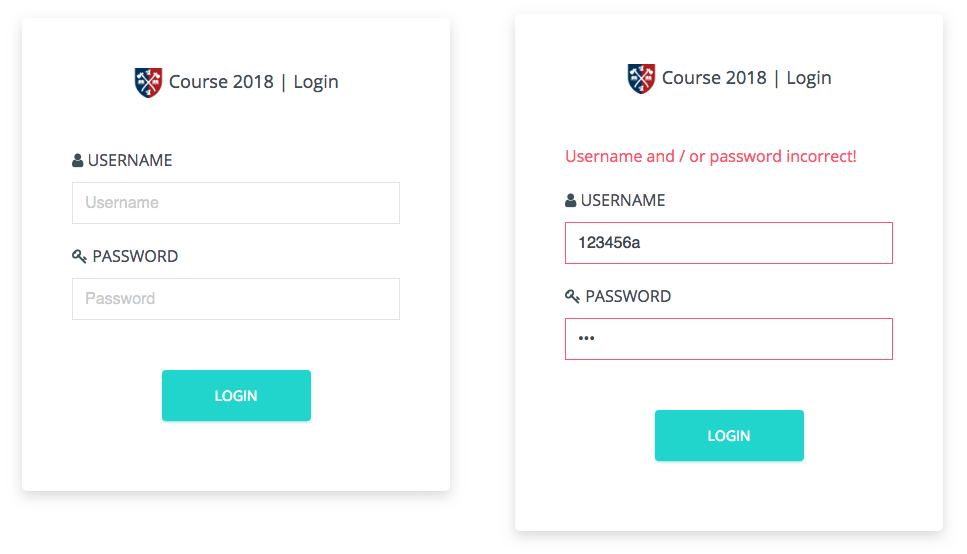
\includegraphics[width=.9\textwidth]{figures/login}
    \caption{System login interface}
    \label{fig:LOGIN}
\end{figure}

\section{Course management}

\subsection{Create courses}
The form shown in Figure~\ref{fig:NEW_COURSE} is used by instructors to create
courses in the \emph{Course\-2018} LMS.

\begin{figure}[H]
    \centering
        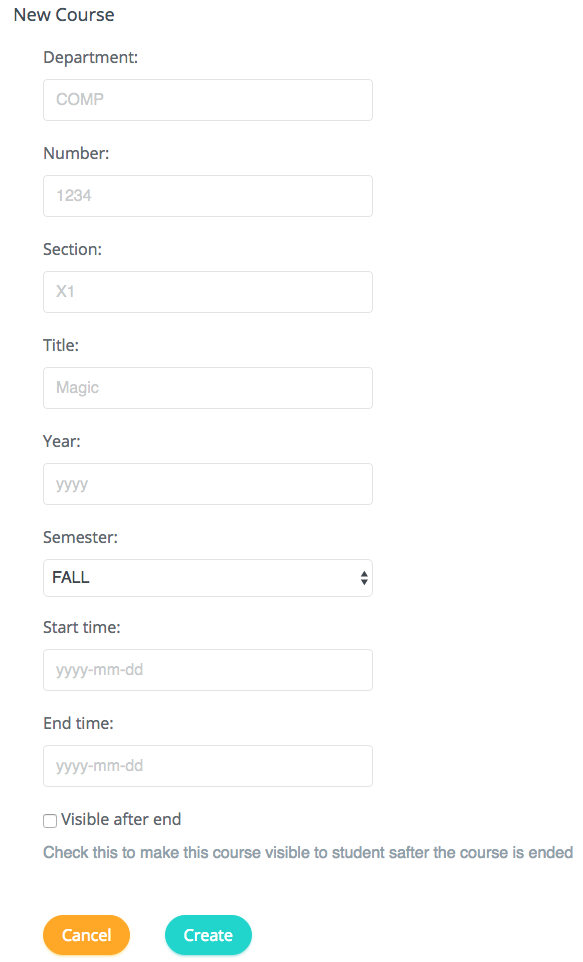
\includegraphics[width=.6\textwidth]{figures/create-courses}
    \caption{Create course interface}
    \label{fig:NEW_COURSE}
\end{figure}

\subsection{Course summary}
Figure~\ref{fig:COURSE_SUMMARY} shows the course summary interface in which
instructors can view the latest assignment grade summary, marking status,
student activities, as well as manage the course (e.g., register TAs, shown
in Figure~\ref{fig:REG_TA}).

The assignment grade summary is a bar chart. Each horizontal bar represents
a problem of an assignment; the length of each bar indicates the number
of students who has submitted that problem; and the proportion of students who
got $[0\%, 20\%)$, $[20\%, 40\%)$, $[40\%, 60\%)$, $[60\%, 80\%)$,
$[80\%, 100\%]$ in each problem is displayed in a different colour in each bar.

\begin{figure}[H]
    \centering
        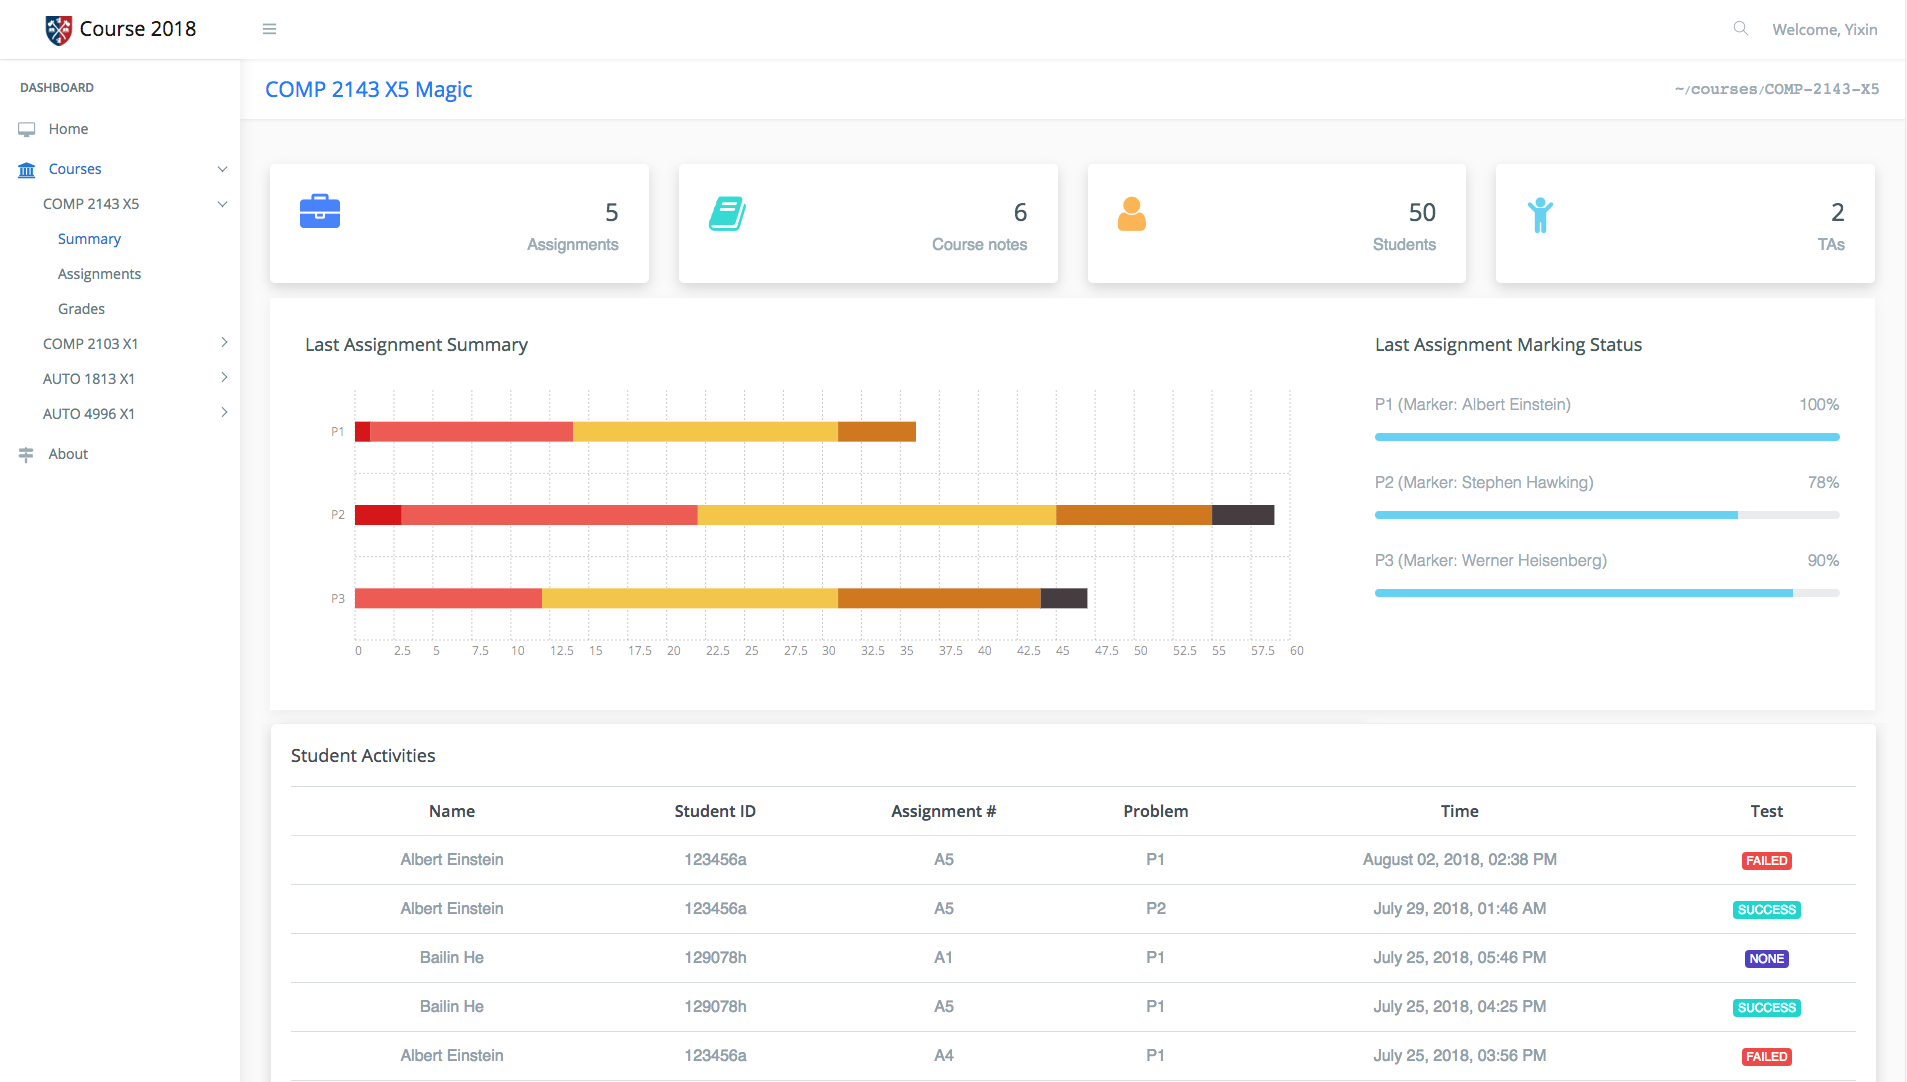
\includegraphics[width=1.0\textwidth]{figures/course-summary}
    \caption{Course summary interface}
    \label{fig:COURSE_SUMMARY}
\end{figure}

\begin{figure}[H]
    \centering
        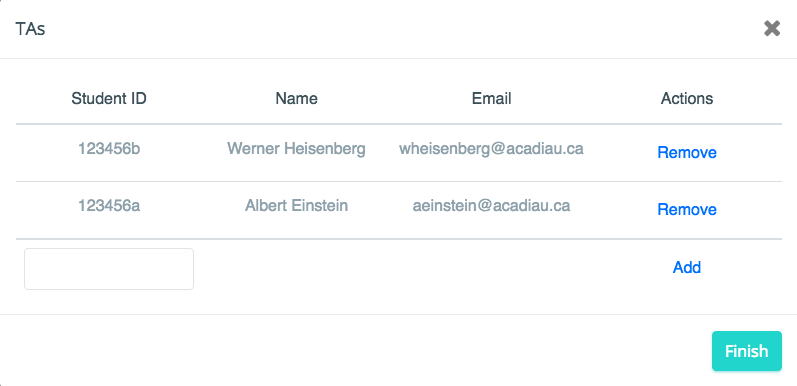
\includegraphics[width=0.8\textwidth]{figures/reg-ta}
    \caption{TA registration interface}
    \label{fig:REG_TA}
\end{figure}


\section{Assignment management}

\subsection{Create assignments}
The form shown in Figure~\ref{fig:NEW_ASM} is used by instructors to create
assignments for a course.

\begin{figure}[H]
    \centering
        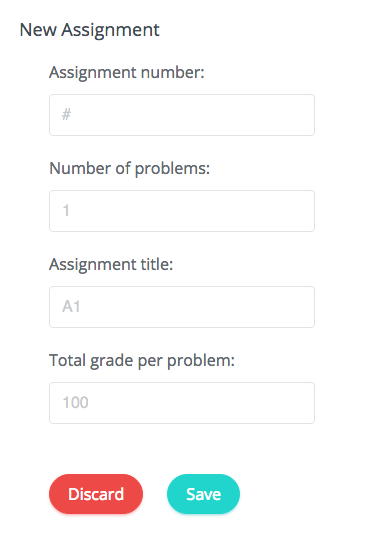
\includegraphics[width=0.4\textwidth]{figures/create-asm}
    \caption{Create assignment interface}
    \label{fig:NEW_ASM}
\end{figure}

\subsection{Assignment summary}

\subsubsection{Professor view}
Figure~\ref{fig:ASM_SUMMARY_PROF} shows the assignment summary interface for
instructors to view the submission status of the latest assignment, manage
each individual assignment, and release assignment feedback to the students.

\subsubsection{Student view}
The student's assignment summary interface, shown in
Figure~\ref{fig:ASM_SUMMARY_STUDENT}, contains a table of a list
of assignments with links to the detail page of each individual assignment.

\begin{figure}[H]
    \centering
        \includegraphics[width=1.0\textwidth]{figures/asm-summary-prof}
    \caption{Assignment summary interface for instructors}
    \label{fig:ASM_SUMMARY_PROF}
\end{figure}

\begin{figure}[H]
    \centering
        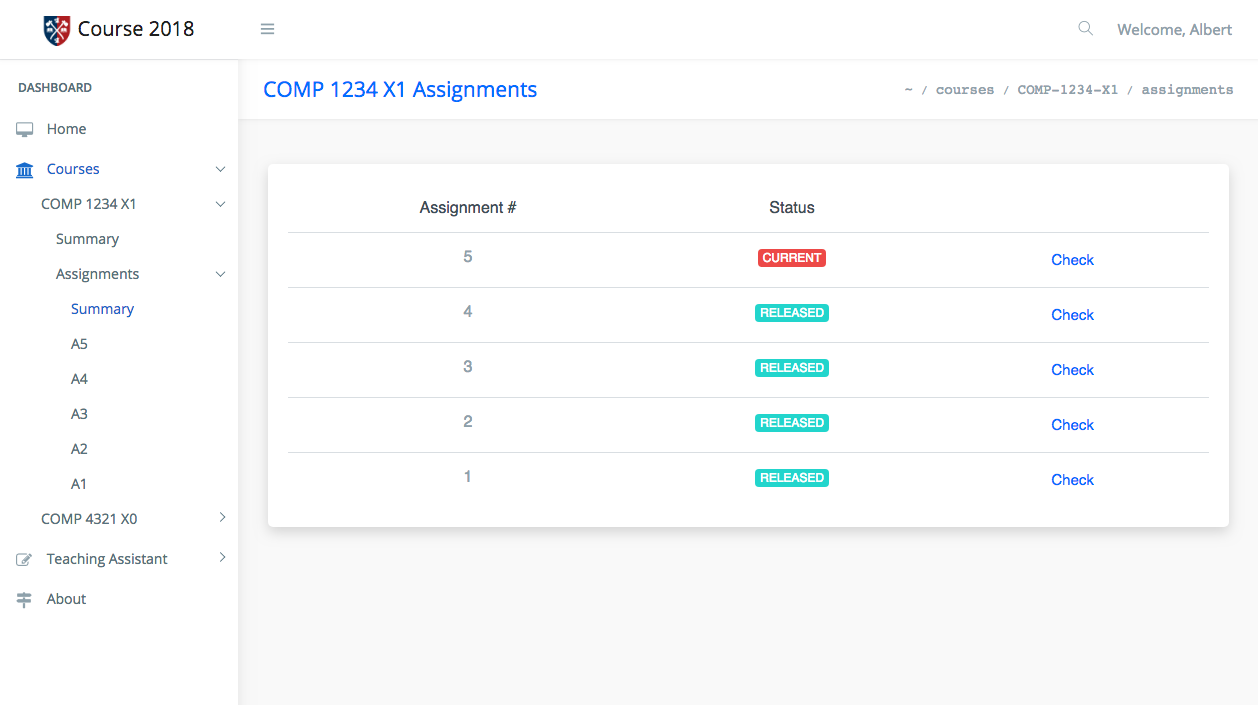
\includegraphics[width=1.0\textwidth]{figures/asm-summary-student}
    \caption{Assignment summary interface for students}
    \label{fig:ASM_SUMMARY_STUDENT}
\end{figure}

\subsection{Assignment detail}

\subsubsection{Professor view}
The assignment detail interface for instructors contains the following three
sections:

\begin{enumerate}
    \item \textbf{Submits}: all submissions of an assignment are displayed
        in a table with links so that instructors can view and grade each
        student's assignment; a drop-down menu is also provided to assign TAs
        to different problems (shown in Figure~\ref{fig:ASM_SUBMITS}).
    \item \textbf{Manage}: the form shown in Figure~\ref{fig:ASM_MANAGE} is
        presented to the instructor in this section
        to modify the detail information of an assignment, as well as to
        manage assignment attachments.
    \item \textbf{Auto Run}: a form (see Figure~\ref{fig:ASM_AUTORUN}) is
        presented to the instructor in this
        section to modify the configurations of the assignment's automated
        test scheme and test cases.
\end{enumerate}

\begin{figure}[H]
    \centering
        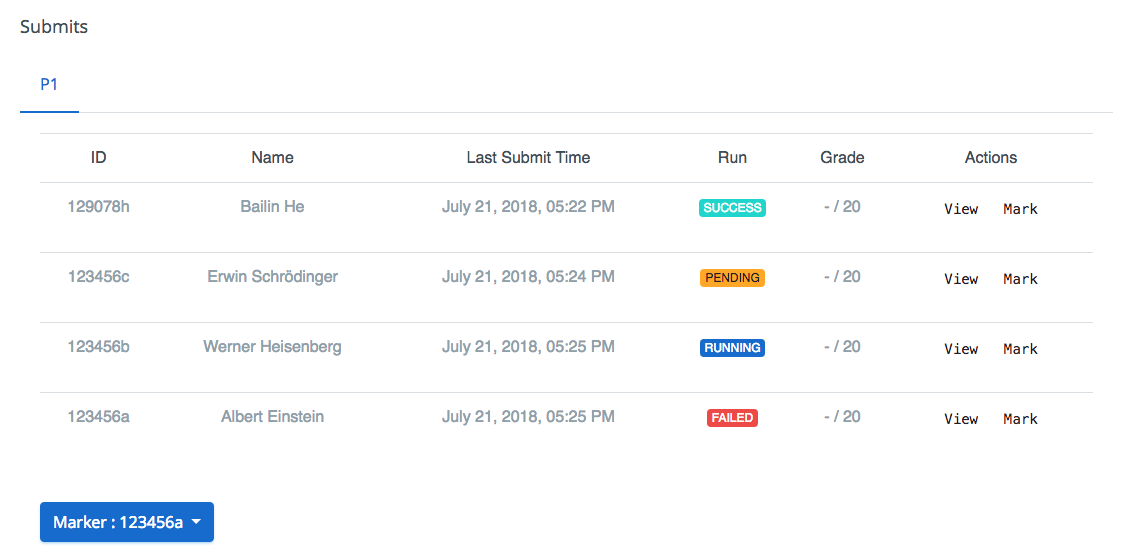
\includegraphics[width=1.0\textwidth]{figures/asm-submits}
    \caption{Assignment submissions interface}
    \label{fig:ASM_SUBMITS}
\end{figure}

\begin{figure}[H]
    \centering
        \includegraphics[width=1.0\textwidth]{figures/asm-manage}
    \caption{Assignment management interface}
    \label{fig:ASM_MANAGE}
\end{figure}

\begin{figure}[H]
    \centering
        \includegraphics[width=0.95\textwidth]{figures/asm-autorun}
    \caption{Assignment automated test configurations interface}
    \label{fig:ASM_AUTORUN}
\end{figure}

\subsubsection{Student View}
The student's assignment detail view is composed of a tab panel where users can
select to view the detail and attachments of an assignment, or submit files
to different problems of an assignment (shown in Figure~\ref{fig:ASM_DETAIL}
and Figure~\ref{fig:ASM_PROBLEM}).

\begin{figure}[H]
    \centering
        \includegraphics[width=1.0\textwidth]{figures/asm-detail}
    \caption{Assignment detail interface for students}
    \label{fig:ASM_DETAIL}
\end{figure}

\begin{figure}[H]
    \centering
        \includegraphics[width=1.0\textwidth]{figures/asm-problem}
    \caption{Assignment problem interface for students}
    \label{fig:ASM_PROBLEM}
\end{figure}


\section{File management and display}

The interface shown in Figure~\ref{fig:FILE_UPLOAD} is used for uploading
attachments (by instructors) and submitting assignments (by students), as well
as management (delete, modify) of those files.

\begin{figure}[H]
    \centering
        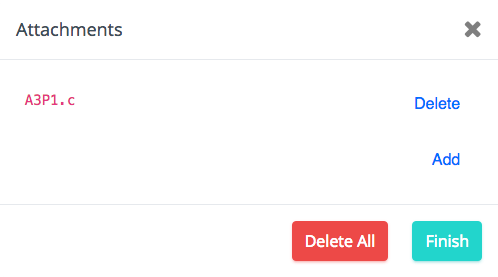
\includegraphics[width=0.7\textwidth]{figures/file-upload}
    \caption{File upload interface}
    \label{fig:FILE_UPLOAD}
\end{figure}

Whenever a user wishes to view a file, the interface shown in
Figure~\ref{fig:VIEW_FILE} is presented to the user. If source code management
(\emph{Git}) is enabled for the assignment, a \emph{Diff} button is displayed;
and the user can click on it to view the changes between the two latest
version of a file, as shown in Figure~\ref{fig:VIEW_FILE_DIFF}.

\begin{figure}[H]
    \centering
        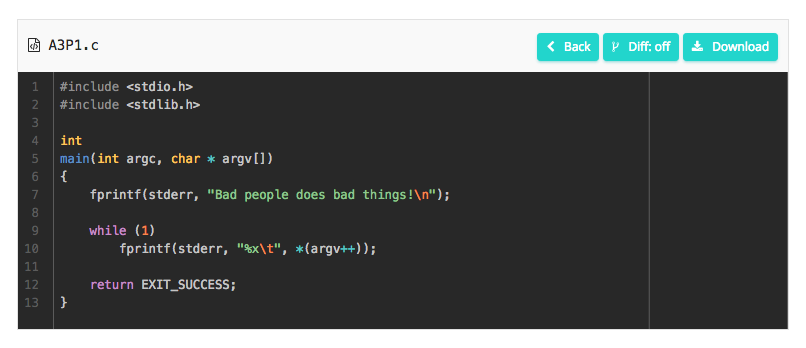
\includegraphics[width=1.0\textwidth]{figures/view-file}
    \caption{File upload interface}
    \label{fig:VIEW_FILE}
\end{figure}

\begin{figure}[H]
    \centering
        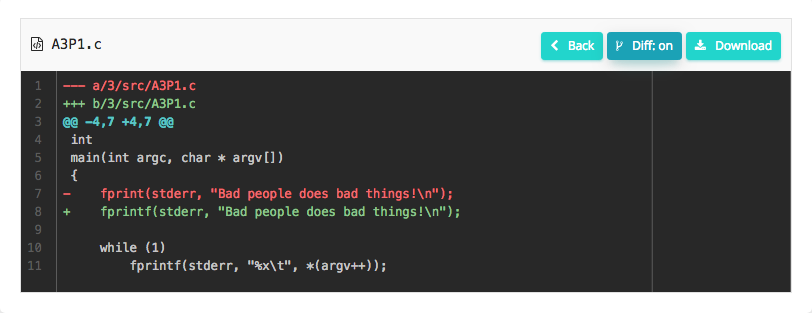
\includegraphics[width=1.0\textwidth]{figures/view-file-diff}
    \caption{File upload interface}
    \label{fig:VIEW_FILE_DIFF}
\end{figure}


\section{Automated test}
As it is shown in Figure~\ref{fig:ASM_SUBMITS} and Figure~\ref{fig:ASM_PROBLEM},
a test status badge is displayed on each submission. This badge is clickable
with a link to an interface that displays the test result
(Figure~\ref{fig:TRACE}).

\begin{figure}[H]
    \centering
        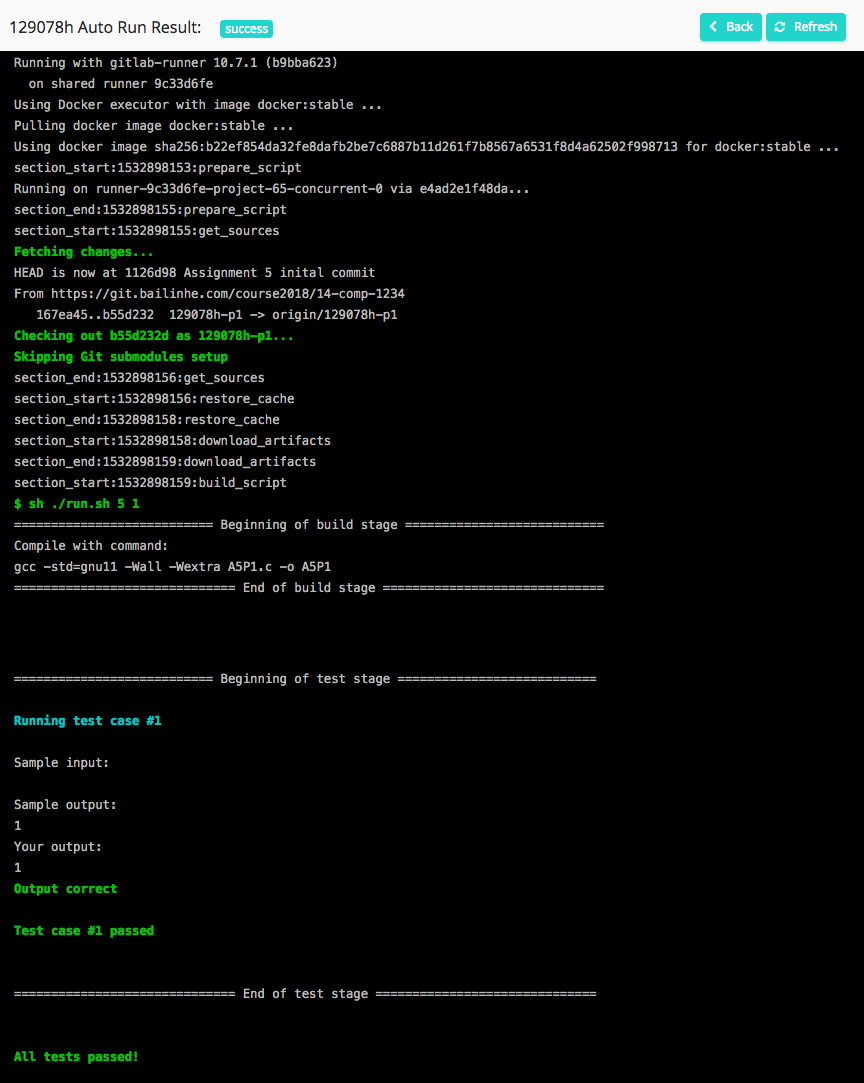
\includegraphics[width=0.85\textwidth]{figures/job-trace}
    \caption{Automated test result interface}
    \label{fig:TRACE}
\end{figure}

If the automated test scheme is updated after a job is finished, a notification
is presented to the user to re-run the test~(Figure~\ref{fig:RERUN}).

\begin{figure}[H]
    \centering
        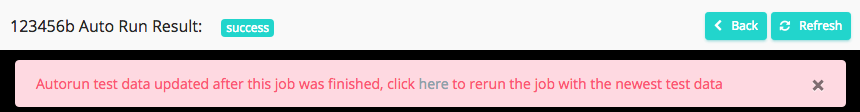
\includegraphics[width=1.0\textwidth]{figures/rerun}
    \caption{Automated test result re-run notification}
    \label{fig:RERUN}
\end{figure}

\section{Marking interface}
\subsection{Marker's view}
The marking interface for markers (i.e., instructors and TAs) is shown in
Figure~\ref{fig:MARKING}. The grade which appears at the upper left corner can
be automatically calculated and updated according to the comments that are
entered in the editor.

\begin{figure}[H]
    \centering
        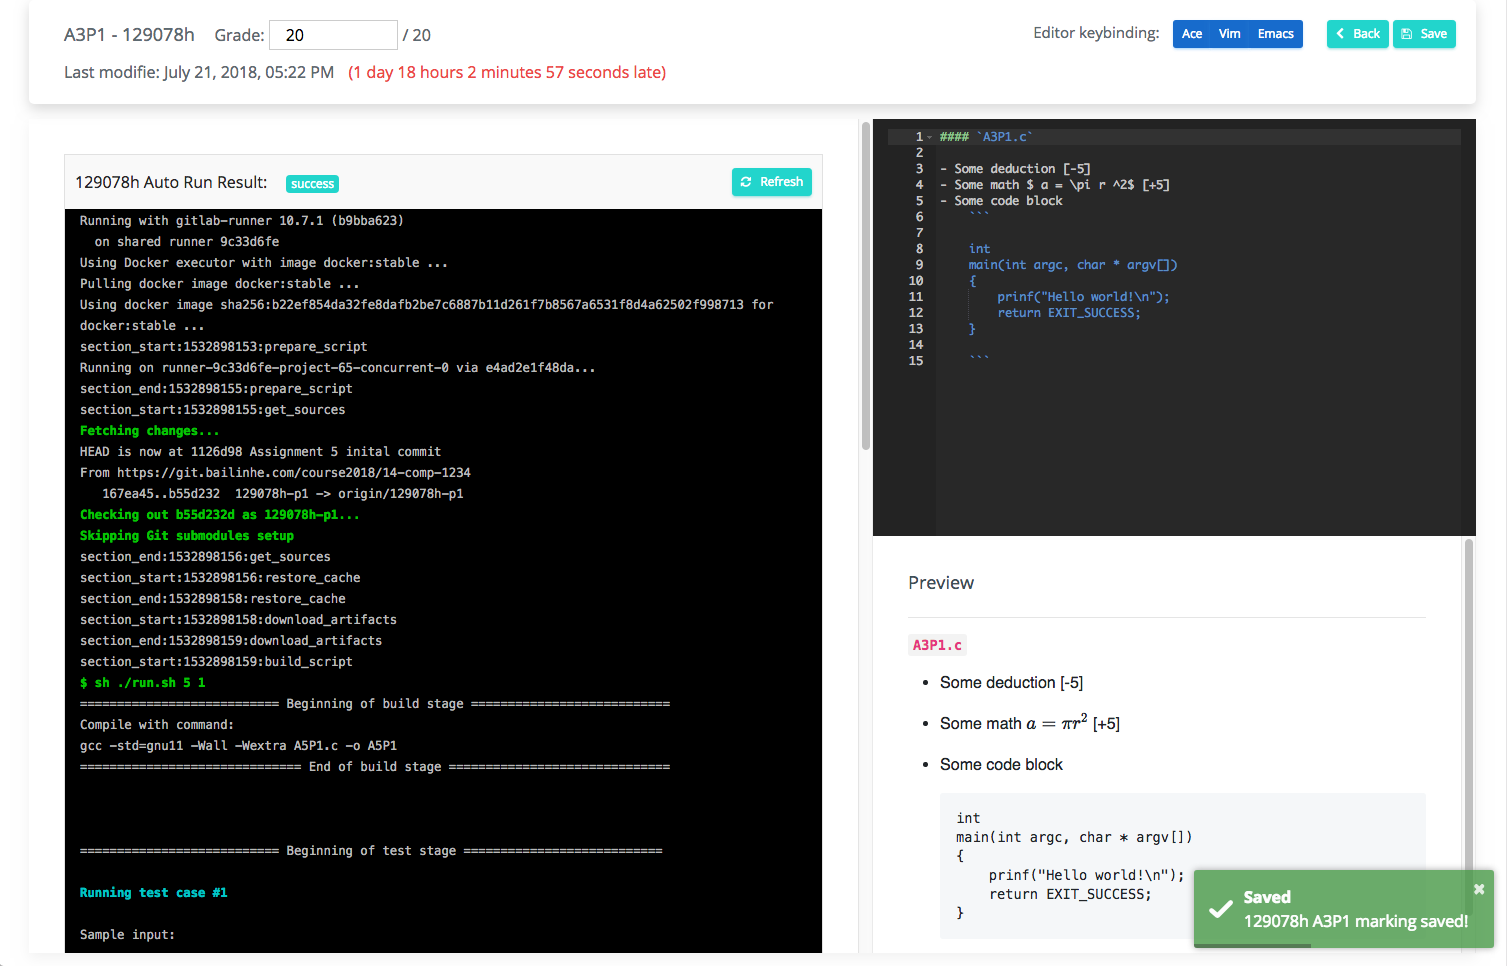
\includegraphics[width=0.95\textwidth]{figures/marker}
    \caption{Marking interface for instructors and TAs}
    \label{fig:MARKING}
\end{figure}

\subsection{Student's view}
The assignment feedback interface for students is shown in
Figure~\ref{fig:FEEDBACK}.
The files of the student's assignment are displayed on the left-hand side,
whereas the TA or instructor's feedback are displayed on the right-hand side,
so that the student can easily refer the comments to his own assignment.

\begin{figure}[H]
    \centering
        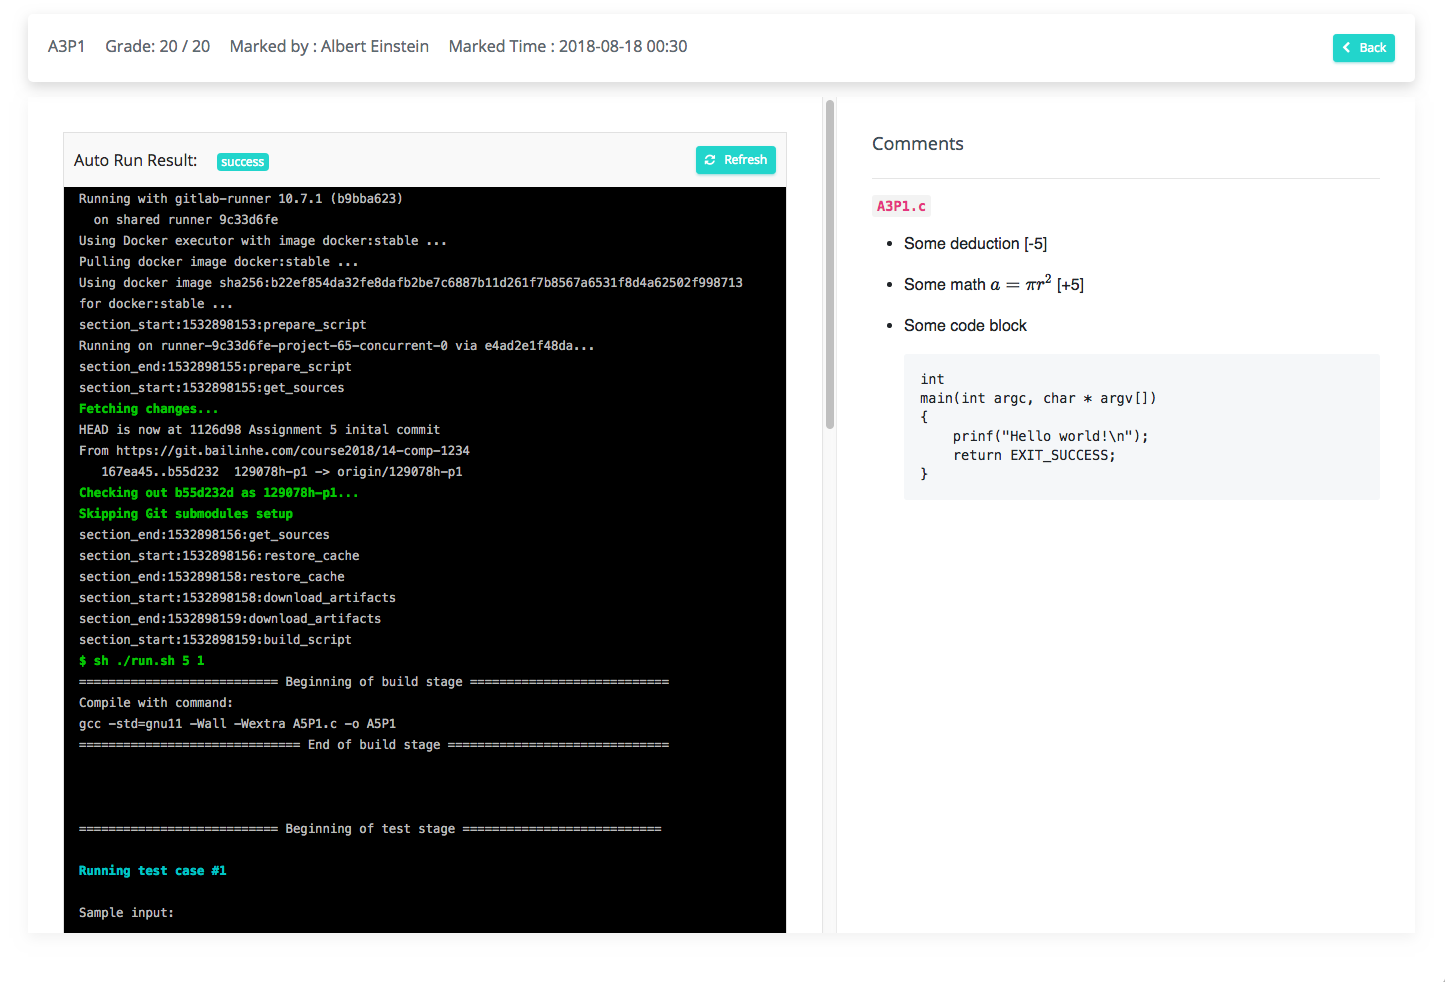
\includegraphics[width=1.0\textwidth]{figures/feedback}
    \caption{Assignment feedback interface for students}
    \label{fig:FEEDBACK}
\end{figure}

    
%-----------------------------------------------------------------------------
% Chapter:Future work 
%-----------------------------------------------------------------------------

\chapter{Future Work and Conclusion}
\label{chap:FUTURE}

\section{Future work}
The \emph{Course2018} LMS has a collection of functionalities 
with features specifically designed for computer science programming
classes.
During the implementation of the code and subsequent testing,
various useful additions to the system
described in the previous chapters were identified.
These additions are described in this chapter.

\subsection{User registration interface}
As of now, the \emph{Course2018} LMS uses the \emph{Django Admin} site to
add new users to the system, but this action can only performed by users that
have \texttt{admin} privilege to the system~\cite{AdjangoAdmin}.
Further, this
makes it very inconvenient to import a large amount of user information to
the system, because all the user information has to be input to the system one
user at a time. Hence, a user registration interface is desired.

\subsubsection{Implementation suggestions}
The user registration should be open only to students
who are registered in courses which are using the \emph{Course2018} LMS\null.
An instructor would first upload a file with the students' basic information
(e.g., student ID, first name, last name, and email) to the LMS\null. The LMS would
create user accounts and profiles for those students, and marks all of them
as inactive users (see attribute \texttt{is\_active} in
Table~\ref{tab:USR_ATTR}).
Then a student can input and submit his student ID to the registration
interface; after the LMS receives the student's ID,
it sends an email with an expirable temporary password to the student's
email account.
Finally, the student uses that temporary password to reset his password and
activate his account.

\subsection{Course materials}
Course material (e.g., lecture notes) management is a desired feature to be
added to the \emph{Course2018} LMS\null.

\subsubsection{Implementation suggestions}
The implementation of this feature should be very simple.
As shown in
Figure~\ref{fig:COURSE_SUMMARY}, the \emph{course summary} template is already
designed to be connected to the course materials management module.
Moreover, the \emph{data model} design of this module should
be very similar to the design of the \emph{AssignmentAttachment} model 
(see Table~\ref{tab:ATTACH_FILE_ATTR}).

\subsection{More source code management functionalities}
Since \emph{Git} and \emph{GitLab} are already integrated to the
\emph{Course2018} LMS, the features listed below can be added to the LMS in the
future with a modest amount of effort:
\begin{itemize}
    \item Revert: allows a user to revert one or more of his submitted files to
        previous versions.
    \item Enhanced version comparison: allows a user to compare the differences
        between any two versions of a file, not just the two most recent
        versions.
    \item Issues: allows a user to post issues (e.g., questions about an
        assignment, or objections to some deductions) on assignments, and
        discuss the issues with the instructor or the TAs.
\end{itemize}

\subsection{Automated test configurations for TAs}
Currently, only instructors are allowed to update automated test
configurations of an assignment in the \emph{Course2018} LMS\null.
It is not uncommon for TAs to come up with new test
cases during the process of grading assignments, and it is desireable for TAs
to have the ability to update the automated test configurations of the
assignment problems they are assigned to grade.

\subsection{\emph{REST} APIs}
Representational State Transfer, also known as \emph{REST}, is a standard of
web applications API architectural style commonly used for communications
between clients and the server~\citep[Chapter 5]{REST}.

To implement all features of the \emph{Course2018} LMS to a set of \emph{REST} APIs
may require a considerable amount of work. However, once this implementation is
finished, the LMS can offer abilities for advanced users to interact with the
LMS in any form they
wish. For example, an instructor can implement a script using those APIs to
interact with the LMS and fully automate the process of assignment management
to satisfy his own workflow. In addition, those sets of APIs can be used
to implement a mobile device version of the \emph{Course2018} application.

\subsection{Interact with the \emph{Moodle} LMS}
A lot of instructors at Acadia University are heavily dependent on the
\emph{Moodle} LMS, for some features that are not provided by
\emph{Course2018} (e.g., grade book, quiz/test tools, and midterm/final
exam grade recording). The efficiency of learning management would be
highly increased if the \emph{Course2018} LMS can interact with the existing
\emph{Moodle} LMS\null.


\section{Conclusion}
In conclusion, this thesis work presents a comprehensive
learning management system which mainly focuses on computer science
programming courses. The implementation of this project demonstrates
a rapid application development process with modern development tools
such as \emph{Docker}, \emph{GitLab}, and \emph{GitLab CI}\null.
The final product, \emph{Course2018} LMS, has the potential to expose
students to a software development environment where features like source
code management and
automated tests play significant roles in their assignments, encouraging
students to submit higher quality work.
Further,
the enhanced marking interface allows professors and TAs to provide more
informative feedback to students in a more efficient way.
    % APPENDICES
    \appendix
    \chapter{Data models implementation}
\label{chap: data-models}


\lstinputlisting[caption=Implementation of the \texttt{UserProfile} model,
label=lst:user-profile,
language=Python
]{./examples/user-profile.py}

\lstinputlisting[caption=Implementation of the \texttt{Course} model,
label=lst:course-model,
language=Python
]{./examples/course-model.py}

\bigskip

\lstinputlisting[caption=Implementation of the \texttt{Assignment} model,
label=lst:assignment-model,
language=Python
]{./examples/assignment-model.py}

\bigskip

\lstinputlisting[caption=Implementation of the \texttt{Commit} model,
label=lst:commit-model,
language=Python
]{./examples/commit-model.py}

\bigskip

\lstinputlisting[caption=Implementation of the \texttt{AutoRun} model,
label=lst:autorun-model,
language=Python
]{./examples/autorun-model.py}
    % \include{another_APPENDIX}
    % CHAPTER CONTENT END

    \bibliography{bibliography/introduction,bibliography/reqs,bibliography/design,bibliography/dev}
\end{document}
